\documentclass[12pt]{article}

% ------------ packages section ------------ 
% page set up
\usepackage{geometry}
\geometry{
 a4paper,
 total={170mm,257mm},
 left=40mm,
 right=25mm,
 top=20mm,
 bottom=25mm
 }
% fonts
\usepackage[T1]{fontenc}
\usepackage{helvet}
% numbering
\usepackage[utf8]{inputenc}
% language set up
\usepackage[portuguese, main=english]{babel}
% line spacing
\usepackage{setspace}
\onehalfspacing
% adjust margins
\usepackage{changepage}
% number lines
\usepackage{lineno}
% titles
\usepackage{titlesec}
% colors
\usepackage[table]{xcolor}
\definecolor{rowgray}{gray}{0.9}
% lorem ipsum generator
\usepackage{blindtext}
\usepackage{array}
\usepackage{booktabs}
% sorted lists package
\usepackage{enumerate}
% insert graphics
\usepackage{graphicx}
% wrapp figures in text
\usepackage{wrapfig}
\usepackage{placeins}
% math package
\usepackage{amsmath}
\usepackage{amssymb} % Required for checkmark symbol
% appendix
\usepackage[title]{appendix}
% letter symbol
\usepackage[misc]{ifsym}
% acronymns
\usepackage[acronym,nonumberlist]{glossaries}
% caption package - settings
\usepackage[font={scriptsize,sf}, labelfont=bf]{caption}
% quotes
\usepackage{csquotes}
\usepackage{dirtytalk}
% BibLaTeX
\usepackage[backend=biber, style=bwl-FU]{biblatex} % style=bwl-FU


% ------------ links setup ------------
\usepackage{hyperref}
\hypersetup{
	colorlinks=true,
	linkcolor=blue,
	citecolor=blue,
	filecolor=magenta,             
	urlcolor=cyan,
	pdftitle={paper sao leo},
	pdfsubject=phd,
	pdfauthor=Ipora Brito Possantti
}


% ------------ page setup ------------
%\pagecolor{black}
%\color{white}

% Set formats for each heading level
\titleformat*{\section}{\Large\bfseries\sffamily}
\titleformat*{\subsection}{\large\bfseries\sffamily}
\titleformat*{\subsubsection}{\normalsize\bfseries\sffamily}


% ------------ listing setup ------------
\usepackage{listings}
\definecolor{codegreen}{rgb}{0,0.6,0}
\definecolor{codegray}{rgb}{0.5,0.5,0.5}
\definecolor{codepurple}{rgb}{0.58,0,0.82}
\definecolor{backcolour}{rgb}{0.95,0.95,0.92}
\lstdefinestyle{mystyle}{
	backgroundcolor=\color{backcolour},  
	commentstyle=\color{gray},
	keywordstyle=\color{brown},
	numberstyle=\tiny\color{codegray},
	stringstyle=\color{codepurple},
	basicstyle=\ttfamily\footnotesize,
	breakatwhitespace=false,              
	breaklines=true,                  
	captionpos=b,                      
	keepspaces=true,                
	numbers=left,                     
	numbersep=2pt,                  
	showspaces=false,              
	showstringspaces=false,
	showtabs=false,                  
	tabsize=3
}
\lstset{style=mystyle}
\renewcommand\lstlistingname{\algname}


% ------------ custom commands ------------
\newcommand{\eqname}{Eq.\,} % equation
\newcommand{\secname}{Sec.\,} % section
\newcommand{\algname}{Alg.} % section
\renewcommand{\figurename}{Fig.\,} % set name of figures
\renewcommand{\tablename}{Tab.\,} % set name of tables


% ------ set metadata ------
\title{\Large{\textsf{\textbf{Streamflow estimation in ungauged catchments using Machine Learning: a nationwide application in Brazil}}}}
\author{\href{https://orcid.org/0000-0002-3910-9244}{Rafael Barbedo}\thanks{\textbf{corresponding author} -- \href{mailto:rbarbedofontana@gmail.com}{\texttt{rbarbedofontana@gmail.com}}, Instituto de Pesquisas Hidráulicas, Federal University of Rio Grande do Sul, Postal Code 15029, Av. Bento Gonçalves, 9500, 91501-970 - Porto Alegre - RS - Brazil} \and \href{https://orcid.org/0000-0002-2194-4516}{Iporã Possantti}\thanks{Instituto de Pesquisas Hidráulicas, Federal University of Rio Grande do Sul} \and \href{https://orcid.org/0000-0002-1053-0131}{Mino Sorribas}\thanks{Instituto de Pesquisas Hidráulicas, Federal University of Rio Grande do Sul} \and \href{https://orcid.org/0000-0003-2918-6681}{Rodrigo Paiva}\thanks{Instituto de Pesquisas Hidráulicas, Federal University of Rio Grande do Sul} \and \href{https://orcid.org/0000-0002-7630-396X}{Walter Collischonn}\thanks{Instituto de Pesquisas Hidráulicas, Federal University of Rio Grande do Sul}}

% set the figure folder
\graphicspath{{./figs}}
% set up labelformat and labelsep for figure
\captionsetup[figure]{labelformat=simple, labelsep=quad}
% add references
\addbibresource{refs.bib}

% ------------ main document ------------
\begin{document}
\pagenumbering{roman}
\maketitle  % fancy title

% abstracts
\begin{adjustwidth}{20pt}{20pt}
\begin{spacing}{0.8}
	\small
	\begin{center}
		\vspace{10mm}
		\textsf{\textbf{Abstract}}
		\vspace{5mm}
	\end{center}
	
	\noindent Knowing river flows in space and time is fundamental for several hydrological and environmental applications. One of the greatest challenges in hydrology, however, is having this information at every river stretch, as we can only focus our resources in obtaining measurements at particular sites. Several research initiatives have been developed over the next years to address this problem, a notorious one being the prediction in ungauged basins (PUB) by the International Association of Hydrological Sciences (IAHS). In recent years, regression techniques based on Machine Learning (\texttt{\texttt{ML}}) approaches have been extensively developed, presenting great results in all areas of knowledge. In hydrological sciences, particularly for PUB, the potential of using these techniques is enormous, and yet, they have not been much explored. In this context, we’ve built a \texttt{ML} regression modelling pipeline, that can be applied to any \texttt{ML} model, to estimate mean annual flows and low flows, and tested it in several different catchments covering the whole of Brazil, using different models to compare the results. We evaluated results against consistent streamflow data from 1069 gauges spread across Brazil that cover distinct characteristics, using 10-fold cross validation, obtaining $R^2$ scores of >0.8 for mean annual flows and >0.7 for low flows. Average and low precipitations were the main drivers for predicting both flow variables. Other important predictors were linked to soil types, land cover, wetlands, and drainage density. \\[2ex]
	
    \noindent \textit{\textbf{keywords}} >>todo: keywords --- Oornare arcu dui; mauris augue; lacus sed turpis.
    \newline
    \newline
    \newline
    \noindent \textit{\textbf{highlights}}:
        >>todo: highlights
        \begin{enumerate}
            \item Tincidunt dui ut ornare lectus sit. Donec adipiscing tristique risus nec feugiat in fermentum posuere urna. Ultricies lacus sed turpis tincidunt id aliquet risus feugiat. 
            \item Ultricies lacus sed turpis tincidunt id aliquet risus feugiat. Ac placerat vestibulum lectus mauris ultrices eros in. Consectetur a erat nam at lectus urna. Enim neque volutpat ac tincidunt vitae semper quis lectus nulla.
            \item Non enim praesent elementum facilisis leo vel. Mauris rhoncus aenean vel elit scelerisque mauris. Rhoncus urna neque viverra justo. 
        \end{enumerate}
\end{spacing}
\clearpage
% --------------- Graphical Abstract ---------------
\begin{center}
    \vspace{10mm}
    \textsf{\textbf{Graphical abstract}}
    \vspace{5mm}
\end{center}
    
\end{adjustwidth}
    
\begin{center}
    
\includegraphics[scale=0.75]{figs/fig.jpg}
\end{center}        
\clearpage

% back to normal size
\normalsize

% table of contents
\tableofcontents
\clearpage    

% list of figures
\listoffigures
\clearpage	

\linenumbers % start line numeration
%\doublespacing % line spacing    
\pagenumbering{arabic} % start arabic numeration
	
\section{Introduction} \label{sec:intro}

\par Understanding river flows in both spatial and temporal domains is crucial for a range of hydrological and environmental applications. Acquiring this data for every river segment is one of the most significant challenges in hydrology. The resources and time required to gauge an entire catchment are substantial, and the costs of setting up and maintaining gauging stations can be exorbitant, particularly in remote or hard-to-access locations. Justifying such investment is challenging in regions with lower data demand. Additionally, environmental or logistical constraints can make gauging a catchment unfeasible, resulting in many catchments worldwide remaining ungauged.

\par The scarcity of river flow data hinders effective decision-making in water resource management. Access to comprehensive flow data could address issues such as over-extraction and water shortages, aid in identifying suitable locations for reservoir construction, and support the implementation of conservation practices to ensure a sufficient water supply for both human use and environmental sustainability. Given the high demand for hydrological data and limited resources for monitoring every catchment, diverse approaches have emerged over the past decades. A notable initiative in this regard is the prediction in ungauged basins (PUB) (\cite{bloschl2013, hrachowitz2013}).

\par One practical approach to mitigate the challenge of data scarcity is the use of reference flows, which simplify the complex behavior of river systems into more manageable metrics. These flows provide insights into a catchment's overall functioning and behavior across different timescales, i.e. its hydrological signature. Commonly used reference flows include median streamflow, low flows, and high flows, representing conditions of water availability, scarcity, or flood risk.

\par Traditionally, reference flows are estimated using discharge regionalization (\cite{laaha2006}). This method involves fitting statistical models to observed data and applying these models to catchments with similar characteristics. While effective in certain contexts, discharge regionalization may not be suitable for large areas with diverse environmental features. In such cases, more sophisticated approaches like process-based hydrological modeling, geostatistical analysis, or advanced statistical models are needed (\cite{bloschl2013}).

\par With recent advancements in world-wide environmental data availability aligned with the development of robust models using Machine Learning (\texttt{ML}), several new horizons are being opened. In hydrological research, these models present great application potential. \texttt{ML} involves developing algorithms based on statistical behaviour of the system, which enables computer systems to learn and make predictions or decisions based on data, without explicit programming. These systems improve performance autonomously based on the input data (\cite{kuhn2013}).

\par The application of \texttt{ML} methods for predicting streamflow in ungauged basins has shown significant potential over the past few years (\cite{ferreira2021, golian2021, potdar2021, worland2018}). The ability of these data-driven methods to learn complex relationships between inputs and outputs allow researchers to gather useful findings that would be substantially challenging with traditional hydrological approaches. Still, further research is necessary to evaluate their reliability and practical applicability.

\par This study aimed to take advantage of the current environmental data availability and those data-driven \texttt{ML} models to produce a nation-wide dataset of average and low reference flows in Brazilian catchments, using streamflow data from various gauges across the country. In order to achieve this, the effectiveness of several \texttt{ML} models in predicting reference flows in ungauged basins were assessed, alongside with the impact of different environmental variables on the predictions and the uncertainty of the estimations associated with them. Based on those evaluations, a comprehensive dataset at this unprecedented scale was produced and made available. In addition to the dataset, a modeling pipeline was established and also made available, incorporating the latest \texttt{ML} modeling techniques, to predict reference average and low flows, using comprehensive environmental data encompassing climate, lithology, and soils.

% Materials and Methods

\section{Data generation description} \label{sec:datagen}

\subsection{Workflow overview}

\par In our study, we structured our workflow to encompass a comprehensive approach to data collection, preparation, processing, modeling, and evaluation. This section and Figure \ref{fig:methods} aim to provide an overview of our workflow, uncovering each step and the methodologies employed. In the following sections, we will delve deeper into each of these steps, offering detailed insights into our methodologies and the rationale behind our choices.

\begin{figure}[t!] % place figure in the page
	\centering                                       
	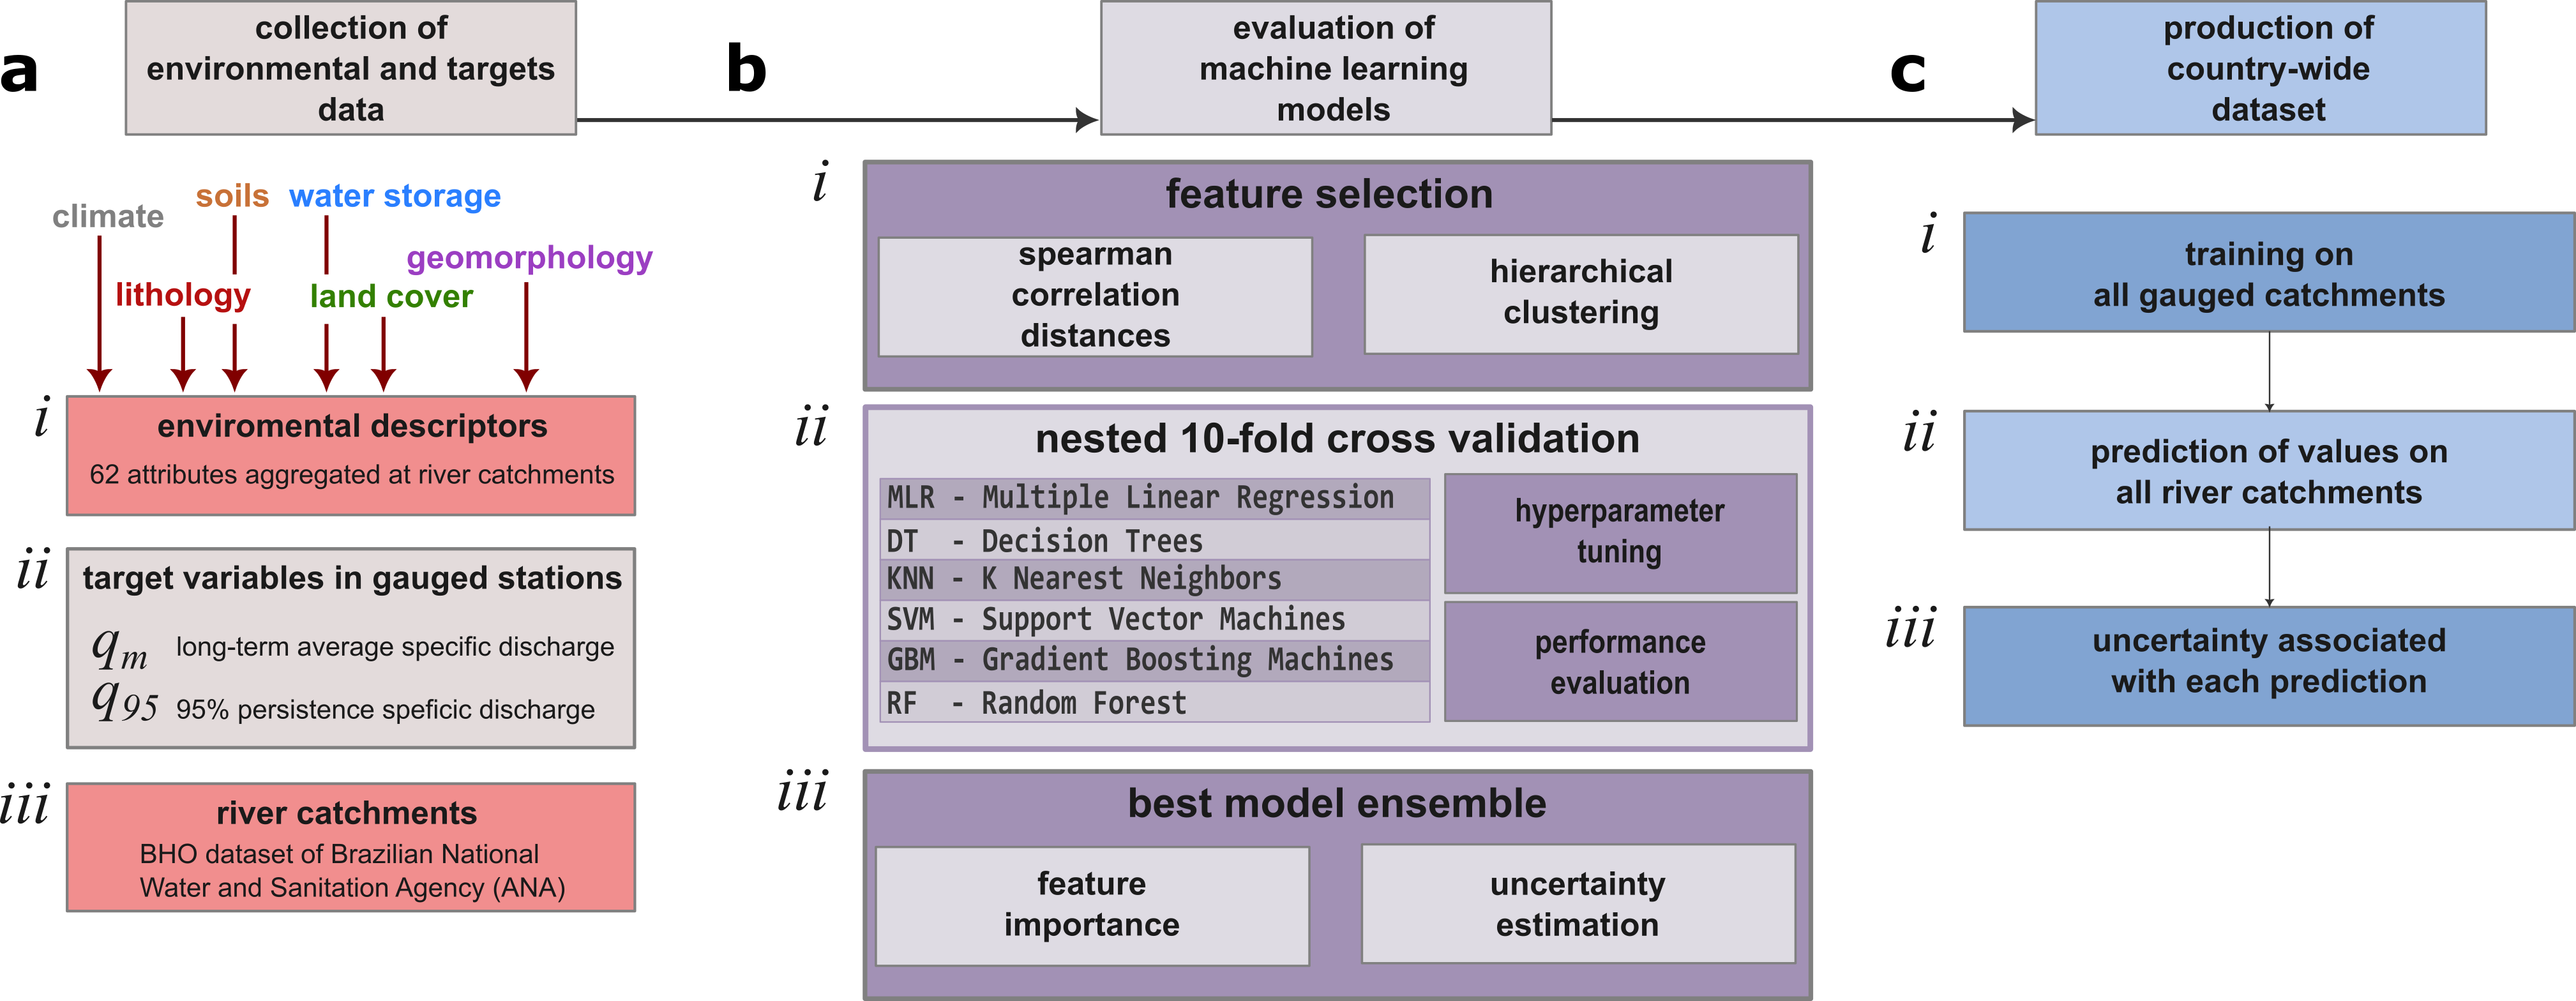
\includegraphics[width=0.98\linewidth]{figs/01_overview.png}    
	\caption[General methodology framework]
	{\textbf{---\;General Workflow for the Proposed Approach}. 
		\textbf{a}\,--\,The workflow began by establishing input datasets. These included environmental descriptors (detail \textrm{\textit{i}}, encompassing data related to climate, soils, lithology, water storage, land cover, and geomorphology), the target variables at gauged stations (detail \textrm{\textit{ii}}, covering long-term average specific discharge $q_m$ and 95\% persistence specific discharge $q_{95}$), and river and basin maps for regionalization (detail \textrm{\textit{iii}}, with data sourced from the BHO dataset \cite{ana2017}).
		\textbf{b}\,--\,The second stage entailed processing and evaluating results. Six Machine Learning models (detail \textrm{\textit{i}}) were fitted following feature selection and hyperparameter tuning (detail \textrm{\textit{ii}}). The evaluation (detail \textrm{\textit{iii}}) focused on model performance metrics, feature importance, and uncertainty assessment.	
        \textbf{c}\,--\,Finally, the output dataset comprised the database of streamflow estimates in ungauged catchments across the entire Brazilian territory (detail \textrm{\textit{i}}) and a consolidated database for the environmental descriptors (detail \textrm{\textit{ii}}).	
	}
	\label{fig:methods}  % use qualitative label                      
\end{figure}

\par We initiated our process with data collection and preparation (section \ref{sec:datagen:input}). For the target variables, we selected river gauges spread across the Brazilian territory based on several criteria to have the most accurate observations available. For the environmental predictors, we focused on gathering a wide range of environmental descriptors that could influence hydrological responses. These descriptors, belonging to the environmental domains of climate, water storage, landscape composition, and topography, were meticulously selected and normalized for consistency across different river basins.

\par Next, we evaluated (1) the performance of six machine learning (ML) models to predict the target data, (2) the influence of each environmental descriptor on the predicted results, and (3) the uncertainty of the predictions (section \ref{sec:datagen:proceval}). For model performance evaluation (1), models tested were Multiple Linear Regression (MLR), Decision Trees (DT), K-Nearest Neighbors (KNN), Support Vector Machines (SVM), Gradient Boosting Machines (GBM), and Random Forest (RF). The pipeline involved first selecting descriptors using hierarchical clustering; then, applying a nested 10-Fold cross-validation approach for training and validating the models, and predicted results of each fold being evaluated using \( BIAS \), \( RMSE \), and \( R^2 \) statistical metrics. For the influence of environmental descriptors (2), the importance of each predictor was assessed using permutation feature importance, which helped us understand the impact of each variable on our models' predictions, enhancing interpretation and understanding of the models. For uncertainty estimation, a careful analysis on the error behaviour was performed on the 3 best performing models (SVM, GBM, and RF), followed by fitting a quantile regression function on the relationship between the errors and the predicted values.

\par Finally, with all the insights provided by the evaluation steps, all of the gauged data was used to train the 3 best models and those trained models were used to predict the reference mean and low flows for catchments linked to each river stretch covering the whole of the Brazilian territory. The dataset covers more than 400k data points, with valuable information on the reference flows that can be used as hydrological signatures of the catchments in Brazil.

% Input data
\subsection{Input data} \label{sec:datagen:input}

% Target variables and delimitation of river basins
\subsubsection{Target variables and river basins} \label{sec:datagen:input:target}

\par Two target variables were analyzed in this study that reflect the long-term behaviour of a catchment within the ambit of water resource management. These variables are the long-term average discharge ($Q_{m}$) and the discharge with a 95\% persistence rate ($Q_{95}$), calculated from daily series of river gauge stations obtained from the Hidroweb database of ANA. Only stations with data series spanning from Jan/1980 to Dec/2014 and containing at least 20 years of data were considered. Furthermore, only stations without significant effects of artificial regulation and/or gross errors in the data series, or of special interest to ANA, were considered. An analysis of estimation errors in long-term discharge associated with sample variability  has demonstrated that estimates based on 20 years of data exhibit errors lower than 5\% in $Q_{m}$ and lower than 15\% in $Q_{95}$ when compared to series of 30 to 35 years in most evaluated cases (\cite{collischonn2021}). Considering these criteria, 1069 stream gauge stations were identified, presented in Figure \ref{fig:rivers}a. For the training and evaluation of the models, the variables used were expressed in specific units ($q_{m}$ and $q_{95}$), dividing the values of $Q_{m}$ and $Q_{95}$ by the area of the upstream basin of each station. Figure \ref{fig:rivers}b illustrate the role of the target variables $q_{m}$ and $q_{95}$ to understand the structure and diversity of  catchment long term behaviour from the inspection of flow duration curves across the Brazilian territory. 

\FloatBarrier
\begin{figure}[htb] % place figure in the page
	\centering                                       
	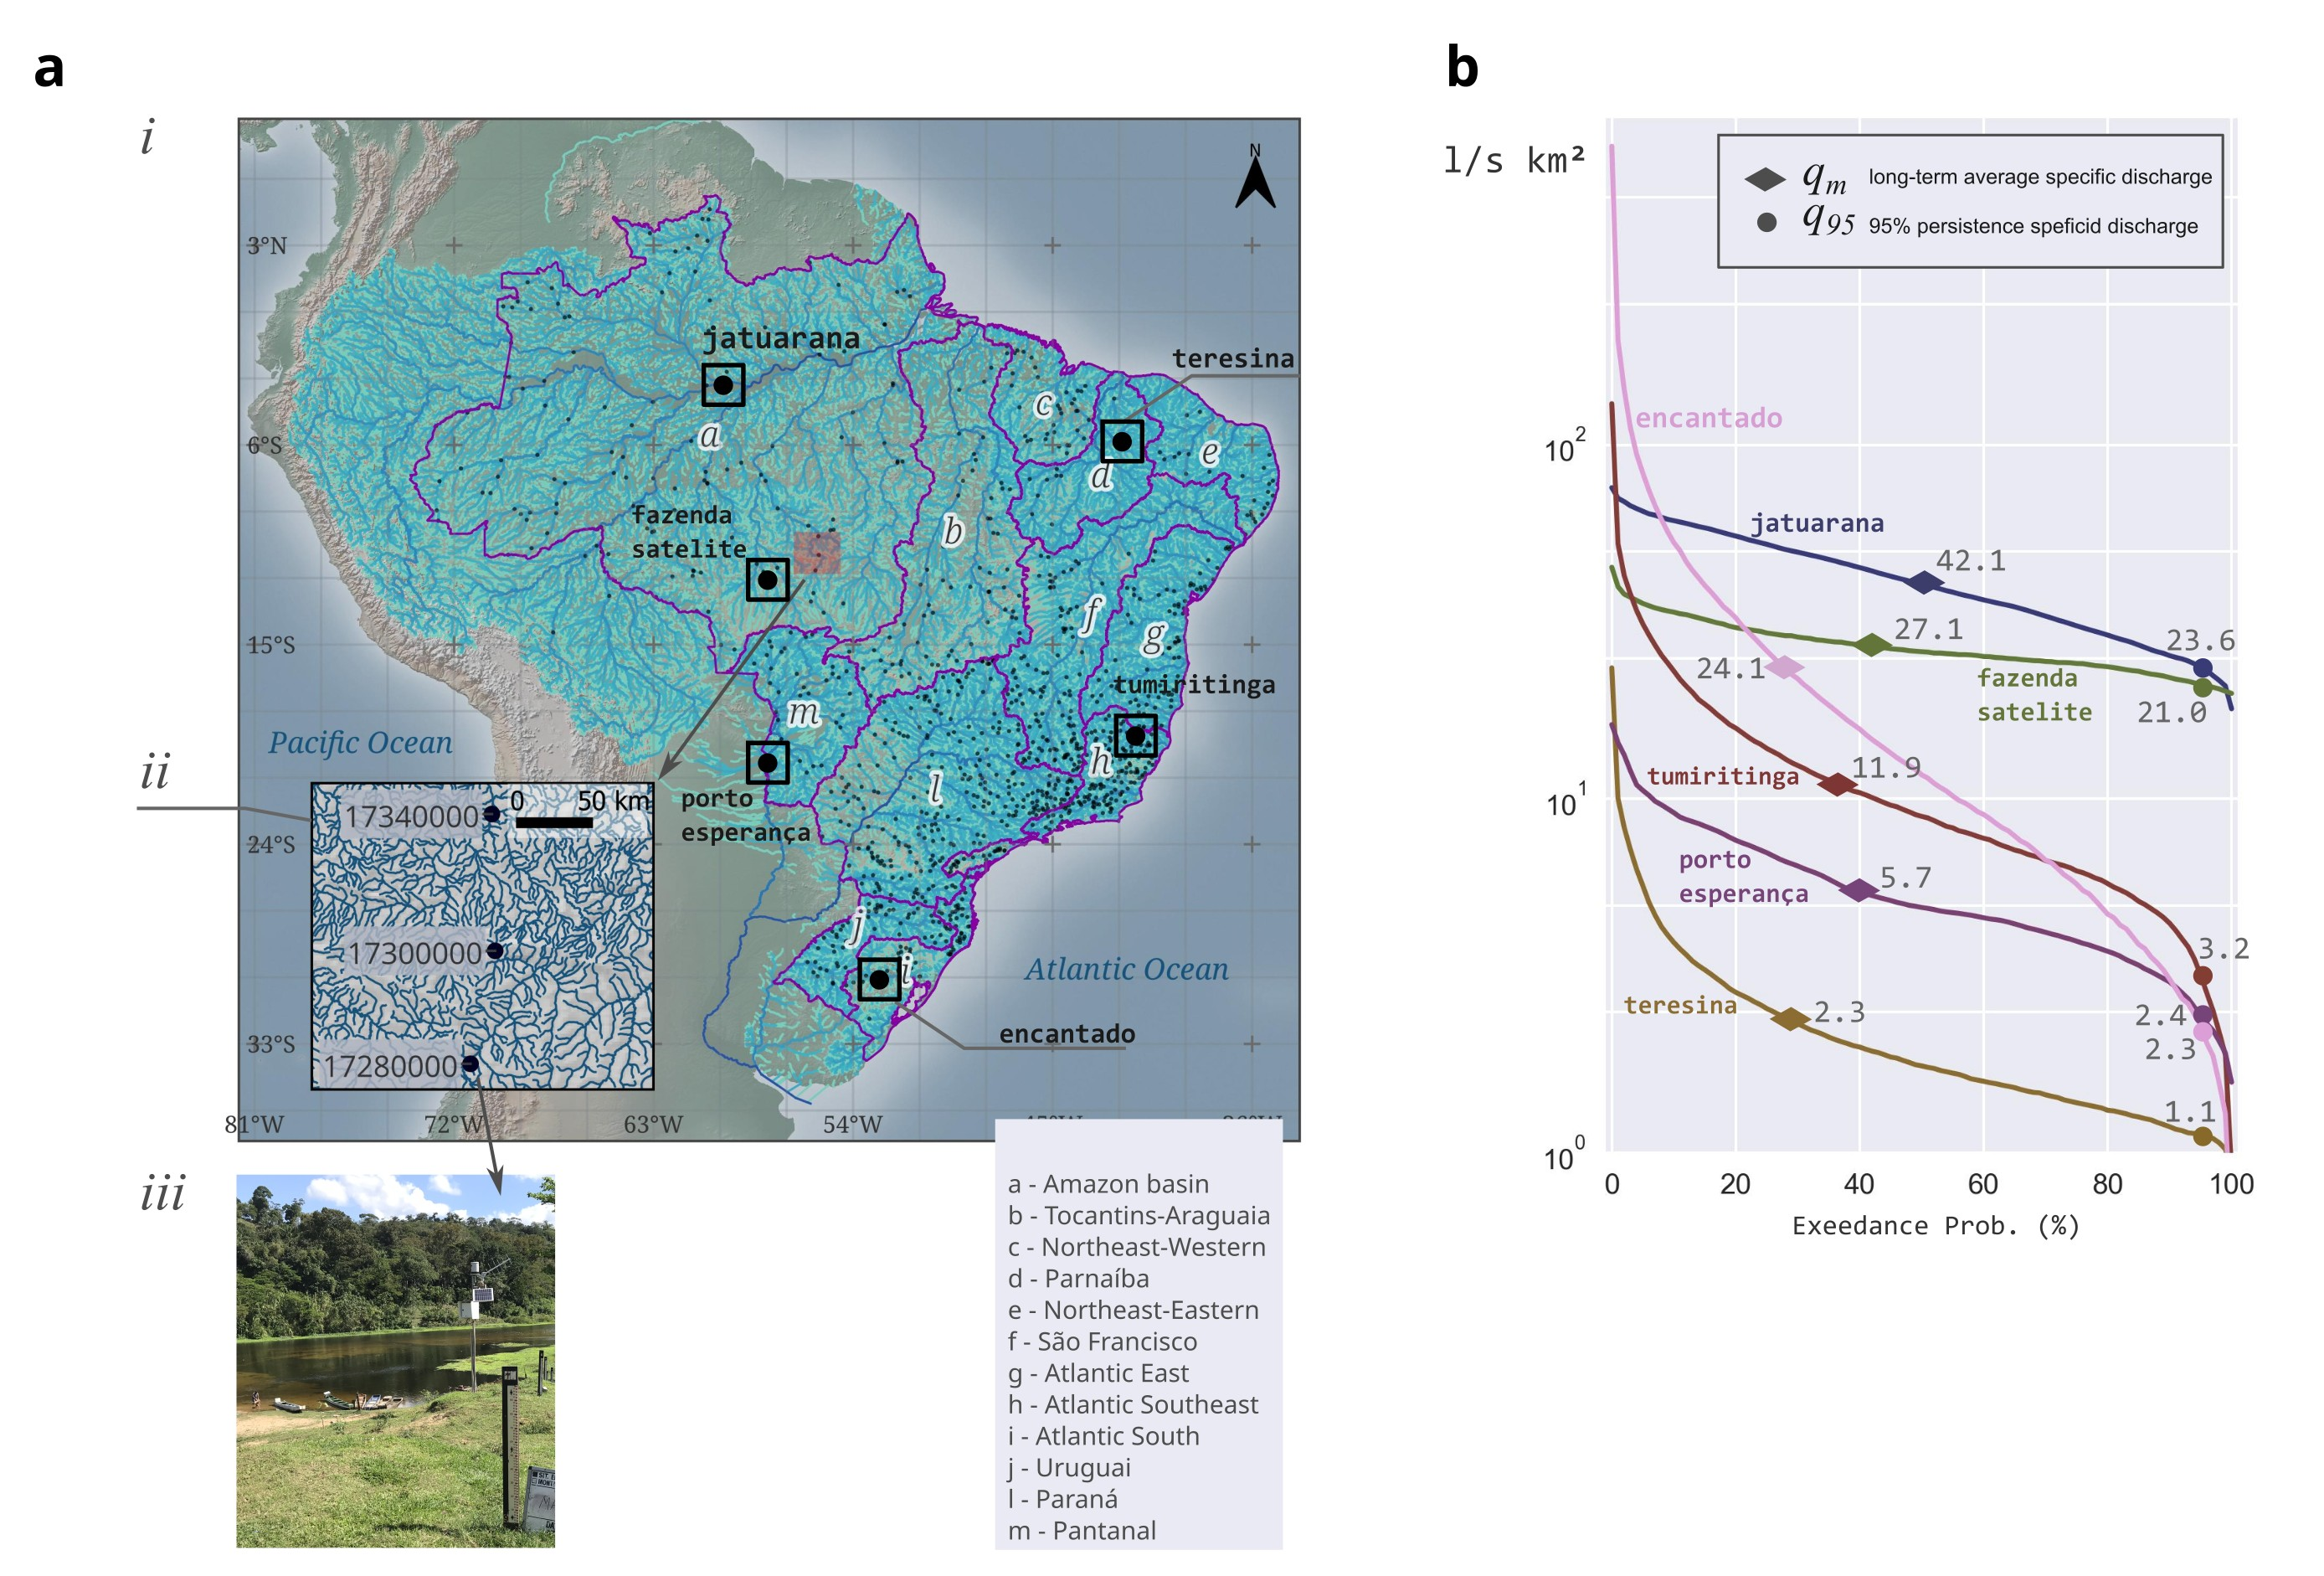
\includegraphics[width=0.98\linewidth]{figs/target.jpg}    
	\caption[Target variables]
	{\textbf{---\;Target variables and locations of the stream gauges used to evaluate the \texttt{ML} models}.
	\textbf{a}\,--\,Map in detail \textrm{\textit{i}} displays the full extent of the Ottocodified hydrological database (\texttt{BHO}) version 5k (\cite{ana2017}), across all Brazilian basins (including contributing areas from neighbouring countries in South America). Detail \textrm{\textit{ii}} uncovers the mapped drainged network and gauged stations. Detail \textrm{\textit{iii}} illustrate the gauged stations operated by Brazilian Geological Survey.
	\textbf{b}\,--\,Illustration of the target variables $q_{m}$ and $q_{95}$ (specific discharge) in flow duration curves in selected stations across the Brazilian territory. The selected stations are also highlighted in \textbf{a}.
	}
    \label{fig:rivers}            
\end{figure}

\par Drainage basins were delimited using the Ottocodified hydrological database (\texttt{BHO}) version 5k (\cite{ana2017}), which was produced by the digitalization of cartographic hydrology data from field surveys produced through decades of development efforts by the Brazilian National Water and Sanitation Agency (ANA) and the Brazilian Institute of Geography and Statistics (IBGE), containing valuable information on Brazilian rivers. It consists of unit catchments in the form of polygons and river lines, with several topological information, making it easy to delimit drainage areas based on the Pfafstetter coding system (\cite{teixeira2022}). For each stream gauge it was defined which unit catchment comprised it (outlet), and them identified all of its upstream unit catchments following the Pfafstetter system. Then, a union operation was performed in all of the polygons, forming the river basin of that station, which was used to collect all data from environmental descriptors. From the \texttt{BHO} dataset, it was also taken drainage area information to be used as a potential predictor.


% Environmental descriptors
\subsubsection{Environmental descriptors datasets} \label{sec:datagen:input:descriptors}

\par We evaluated 62 variables of environmental descriptors with potential to influence the hydrological response of a river basin. These variables were selected based on environmental characteristics with potential to describe catchment behaviour and, therefore, streamflow response. Here, they were grouped in domains of climate, water storage, landscape composition, and topography. A summary of all variables is presented in Table \ref{tab:predictors}. Next, a brief description of the variables and datasets used is given.

% Insert Table Predictors
\FloatBarrier
\begin{table}[htb]
\centering
\tiny
\rowcolors{2}{white}{rowgray}
\begin{tabular}{p{0.5cm}p{1cm}p{2cm}p{3.5cm}p{5cm}}
\toprule
\textbf{Code} & \textbf{Notation} & \textbf{Domain} & \textbf{Description} & \textbf{Source} \\
\midrule
1 & $P_{avg}$ & Climate & Precipitation average & Remote Sensing -- \texttt{IMERG}\\
2 & $P_{min}$ & Climate & Precipitation minimum & Remote Sensing -- \texttt{IMERG}\\
3 & $P_{max}$ & Climate & Precipitation maximum & Remote Sensing -- \texttt{IMERG}\\
4 & $T_{avg}$ & Climate & Temperature average & Remote Sensing -- \texttt{MODIS}\\
5 & $T_{min}$ & Climate & Temperature minimum & Remote Sensing -- \texttt{MODIS}\\
6 & $T_{max}$ & Climate & Temperature maximum & Remote Sensing -- \texttt{MODIS}\\
7 & $ET_{avg}$ & Climate & Evapotranspiration average & Remote Sensing -- \texttt{MODIS}\\
8 & $ET_{min}$ & Climate & Evapotranspiration minimum & Remote Sensing -- \texttt{MODIS}\\
9 & $ET_{max}$ & Climate & Evapotranspiration maximum & Remote Sensing -- \texttt{MODIS}\\
10 & $PET_{avg}$ & Climate & Potential Evapot. average & Remote Sensing -- \texttt{MODIS}\\
11 & $PET_{min}$ & Climate & Potential Evapot. minimum & Remote Sensing -- \texttt{MODIS}\\
12 & $PET_{max}$ & Climate & Potential Evapot. maximum & Remote Sensing -- \texttt{MODIS}\\
13 & $WS_{rs}$ & Water Storage & Reservoir storage & \texttt{SIN}  -- \cite{barbedo2022ws}\\
14 & $WS_{sw}$ & Water Storage & Surface water & \texttt{MGB-SA} -- \cite{barbedo2022ws}\\
15 & $WS_{sm}$ & Water Storage & Soil Moisture & \texttt{GLDAS} -- \cite{barbedo2022ws}\\
16 & $WS_{gw}$ & Water Storage & Groundwater storage & \texttt{Various} -- \cite{barbedo2022ws}\\
17 & $WS_{tt}$ & Water Storage & Total & GRACE -- \cite{barbedo2022ws}\\
18 & $LT_{ev}$ & Lithology & Evaporites & \texttt{GLiM}  -- \cite{hartmann2012}\\
19 & $LT_{ig}$ & Lithology & Ice and Glaciers & \texttt{GLiM}  -- \cite{hartmann2012}\\
20 & $LT_{mt}$ & Lithology & Metamorphics & \texttt{GLiM}  -- \cite{hartmann2012}\\
21 & $LT_{nd}$ & Lithology & No Data & \texttt{GLiM}  -- \cite{hartmann2012}\\
22 & $LT_{pa}$ & Lithology & Acid plutonic rocks & \texttt{GLiM}  -- \cite{hartmann2012}\\
23 & $LT_{pb}$ & Lithology & Basic plutonic rocks & \texttt{GLiM}  -- \cite{hartmann2012}\\
24 & $LT_{pi}$ & Lithology & Intermediate plutonic rocks & \texttt{GLiM}  -- \cite{hartmann2012}\\
25 & $LT_{py}$ & Lithology & Pyroclastics & \texttt{GLiM}  -- \cite{hartmann2012}\\
26 & $LT_{sc}$ & Lithology & Carbonate sed. rocks & \texttt{GLiM}  -- \cite{hartmann2012}\\
27 & $LT_{sm}$ & Lithology & Mixed sedimentary rocks & \texttt{GLiM}  -- \cite{hartmann2012}\\
28 & $LT_{ss}$ & Lithology & Siliciclastic sed. rocks & \texttt{GLiM}  -- \cite{hartmann2012}\\
29 & $LT_{su}$ & Lithology & Unconsolidated sediments & \texttt{GLiM}  -- \cite{hartmann2012}\\
30 & $LT_{va}$ & Lithology & Acid volcanic rocks & \texttt{GLiM}  -- \cite{hartmann2012}\\
31 & $LT_{vb}$ & Lithology & Basic volcanic rocks & \texttt{GLiM}  -- \cite{hartmann2012}\\
32 & $LT_{vi}$ & Lithology & Intermediate volcanic rocks & \texttt{GLiM}  -- \cite{hartmann2012}\\
33 & $LT_{wb}$ & Lithology & Water Bodies & \texttt{GLiM}  -- \cite{hartmann2012}\\
34 & $SC_{wtr}$ & Soil content & Soil water content (g/g) & \texttt{OpenLandMap} -- \cite{hengl2017}\\
35 & $SC_{cly}$ & Soil content& Soil organic content (g/g) & \texttt{OpenLandMap} -- \cite{hengl2017}\\
36 & $SC_{org}$ & Soil content & Soil sand content (g/g) & \texttt{OpenLandMap} -- \cite{hengl2017}\\
37 & $SC_{snd}$ & Soil content & Soil clay content (g/g) & \texttt{OpenLandMap} -- \cite{hengl2017}\\
38 & $ST_{cl}$ & Soil texture & Clay & \texttt{OpenLandMap}  -- \cite{hengl2017}\\
39 & $ST_{sicl}$ & Soil texture & Silty clay & \texttt{OpenLandMap}  -- \cite{hengl2017}\\
40 & $ST_{sacl}$ & Soil texture & Sandy clay & \texttt{OpenLandMap}  -- \cite{hengl2017}\\
41 & $ST_{cllo}$ & Soil texture & Clay loam & \texttt{OpenLandMap}  -- \cite{hengl2017}\\
42 & $ST_{sicllo}$ & Soil texture & Silty clay loam & \texttt{OpenLandMap}  -- \cite{hengl2017}\\
43 & $ST_{sacllo}$ & Soil texture & Sandy clay loam & \texttt{OpenLandMap}  -- \cite{hengl2017}\\
44 & $ST_{lo}$ & Soil texture & Loam & \texttt{OpenLandMap}  -- \cite{hengl2017}\\
45 & $ST_{siso}$ & Soil texture & Silty loam & \texttt{OpenLandMap}  -- \cite{hengl2017}\\
46 & $ST_{salo}$ & Soil texture & Sandy loam & \texttt{OpenLandMap}  -- \cite{hengl2017}\\
47 & $ST_{si}$ & Soil texture & Silt & \texttt{OpenLandMap}  -- \cite{hengl2017}\\
48 & $ST_{losa}$ & Soil texture & Loamy sand & \texttt{OpenLandMap}  -- \cite{hengl2017}\\
49 & $ST_{sa}$ & Soil texture & Sand & \texttt{OpenLandMap}  -- \cite{hengl2017}\\
50 & $LC_{fr}$ & Land Cover & Forest & \texttt{Mapbiomas} -- \cite{souza2020} and \texttt{MODIS}\\
51 & $LC_{gr}$ & Land Cover & Grassland & \texttt{Mapbiomas} -- \cite{souza2020} and \texttt{MODIS}\\
52 & $LC_{ag}$ & Land Cover & Agriculture & \texttt{Mapbiomas} -- \cite{souza2020} and \texttt{MODIS}\\
53 & $LC_{pr}$ & Land Cover & Semi-permeable & \texttt{Mapbiomas} -- \cite{souza2020} and \texttt{MODIS}\\
54 & $LC_{wt}$ & Land Cover & Water & \texttt{Mapbiomas} -- \cite{souza2020} and \texttt{MODIS}\\
55 & $TP_{elv}$ & Geomorphology & Elevation average & \texttt{MERIT} -- \cite{yamazaki2017}\\
56 & $TP_{slp}$ & Geomorphology & Slope average & \texttt{MERIT} -- \cite{yamazaki2017}\\
57 & $TP_{hnd}$ & Geomorphology & HAND average & Produced\\
58 & $TP_{dd}$ & Geomorphology & Drainage density & Produced\\
59 & $TP_{ua}$ & Geomorphology & Upstream area & \texttt{BHO 5k} -- \cite{ana2017}\\
60 & $TC_{wtl}$ & Geomorphology & Wetland & Produced\\
61 & $TC_{hls}$ & Geomorphology & Hillslope & Produced\\
62 & $TC_{plt}$ & Geomorphology & Plateau & Produced\\
\bottomrule
\end{tabular}
\caption{Environmental predictors used as input for the \texttt{ML} models.}
\label{tab:predictors}
\end{table}

\begin{itemize}
    \item Climate
\end{itemize}

\par Climate-related variables such as precipitation, temperature, evapotranspiration, and potential evapotranspiration, were normalized to monthly averages from 2001 to 2020 for each river basin, using minimum, maximum, and average values. Precipitation was sourced from the Integrated Multi-Satellite Retrievals for \texttt{GPM} (\texttt{IMERG}), a product of \texttt{NASA} and \texttt{JAXA} (\cite{huffman2020}). \texttt{IMERG} provides high-resolution global precipitation estimates, combining data from satellites like \texttt{TRMM} (\cite{huffman2007}) and the \texttt{GPM} mission (\cite{skofronick2017}). Land surface temperature (\textit{T}), evapotranspiration (\textit{ET}), and potential evapotranspiration (\textit{PET}), were collected from the Moderate Resolution Imaging Spectroradiometer (\texttt{MODIS}) products (\cite{mu2007, mu2011i}), derived from the Terra and Aqua satellites. These variables play a significant role in the water loss processes and are key to understanding streamflow responses in basins.

\begin{itemize}
    \item Water Storage
\end{itemize}

\par Different components of water storage such as groundwater, soil moisture, surface water, and reservoir water were also included in the list of enviromental descriptors, with data collection methods detailed in \cite{barbedo2022a}. Total water storage data was derived from the Gravity Recovery and Climate Experiment (\texttt{GRACE}) and its follow-up mission \texttt{GRACE-FO}, which measure changes in Earth's gravity field due to water mass distribution shifts (\cite{landerer2020, tapley2004}). Reservoir storage information came from the Brazilian National Interconnected System (SIN), providing insights into reservoir capacities and water levels (\cite{ana2021}). Surface water storage data was acquired from the \texttt{MGB-SA} hydrological model, a physically-based framework that simulates the hydrological cycle of Brazilian river basins and includes rivers, lakes, and wetlands (\cite{siqueira2018}). Soil moisture data, crucial for understanding plant water uptake, was sourced from the Global Land Data Assimilation System (\texttt{GLDAS}), which assimilates various data to estimate soil moisture globally, particularly in the root zone (\cite{rodell2004}).

\begin{itemize}
    \item Lithology, Soils, and Land Cover
\end{itemize}

\par The categorical variables belonging to the domains of lithology, soils, and land cover were collected based on the percentage of occupancy of each class within basin boundaries. Variables related to soil content were numerical (water, organic matter, clay, silt, and sand contents), which were averaged over basin areas. Lithology classes came from the Global Lithological Map (\texttt{GLiM}) database (\cite{hartmann2012}). This database, at a 50km resolution, gets geological information from various sources to categorize the Earth's surface into ten lithological classes, including sedimentary, volcanic, plutonic, metamorphic rocks, and unconsolidated deposits. Soil properties were sourced from the \texttt{OpenLandMap} database (\cite{hengl2017}). This database consists of detailed global soil information at 250m resolution, including texture, organic matter content, and pH, utilizing a blend of soil maps and modelling. For land cover classes, data from the \texttt{Mapbiomas} database (\cite{souza2020}) was used for Brazilian territory and the \texttt{MODIS} dataset (\cite{friedl201}) for the remaining areas. Both databases' original land cover classes were simplified into five categories: forests, grasslands, agriculture, semi-permeable regions, and water bodies, facilitating cross-regional analysis and comparison.

\begin{itemize}
    \item Geomorphology
\end{itemize}

\par Geomorphological variables, in here, were considered as all variables derived from a digital elevation model (\texttt{DEM}); some requiring minimal processing, like elevation and slope, and others needing more complex procedures, such as drainage networks and terrain class attributions. Elevation and slope data for each river basin, including averages and standard deviations, were obtained from the \texttt{MERIT-DEM} product (\cite{yamazaki2017}), which consists of a \texttt{DEM} with approximately 90 m resolution, derived by correcting vegetation height errors from other \texttt{DEM} datasets. For drainage-dependent information, we used the Topographic Position based Stream definition (\texttt{TPS}) (\cite{barbedo2022b}) to generate a stream mask using \texttt{MERIT-DEM} and \texttt{MERIT-Hydro} (\cite{yamazaki2019}). From the combination of the derived drainage with the \texttt{DEM}, a Height Above Nearest Drainage (\texttt{HAND}) map was created (\cite{nobre2011, renno2008}), providing insights into drainage density and water table depth across river basins. From these maps, it was also computed a categorical map by classifying the landscape into three hydrological classes: wetlands, hillslopes, and plateaus. This classification is based on several studies linking terrain and drainage attributes to hydrological response (e.g. \cite{gao2014, gharari2011, savenije2010}), and it was obtained from drainage locations and \texttt{DEM} data, where wetlands are identified using a \texttt{HAND} threshold below which the area is most of the time saturated (5m was the value used here); hillslopes, by a slope threshold above which faster water movements and erosion are dominant (10\% was the value used here); and plateaus, falling in between the former maps, and represent areas generally higher and flatter where groundwater recharge is more present.

% Machine Learning algorithms
\subsection{Evaluation of models} \label{sec:datagen:proceval}

\par \textcolor{red}{!! Figura com nested K-Folds | processing overview}


% Feature selection
\subsubsection{Feature selection} \label{sec:datagen:proceval:selection}

\par From the 62 initial variables, we first excluded the ones with no values in the catchments analyzed ($ST_{Si}$, $LT_{Ev}$, and $LT_{Ig}$), ending up with 59 environmental descriptors. On those, hierarchical clustering was employed for feature selection, as described by \cite{johnson1967}. This technique involves grouping similar data points into clusters, visualized through a dendrogram, a tree-like structure. In feature selection, hierarchical clustering aids in identifying groups of similar features for potential combination or removal. The process begins with the creation of a correlation matrix, using the Spearman correlation coefficient to capture non-linear relationships among variables. This matrix displays pairwise correlations between all features. Following this, features were clustered based on their pairwise correlation single-link distances. The dendrogram helped in deciding the level at which to cut and form the final feature clusters. The number of clusters chosen depended on the chosen dendrogram cut-off distance.

\par Feature selection within each cluster was then carried out. The representative feature was determined as the one with the highest correlation to the target variable. This approach varied for each target variable (\( q_{m} \) and \( q_{95} \)), ensuring the selection of the most relevant features. The process of selecting the cutting threshold for the dendrogram was iterative, focusing on model performance and ensuring the remaining features were representative of the dataset and not correlated between each other, with the criteria focusing on maintaining features with pairwise Spearman absolute correlation below 0.75, and with no decrease in model performance on predicted values. This method ensured the inclusion of the most representative variables while avoiding multi-collinearity, balancing representativeness and analytic integrity. Thus, by using a distance threshold of 0.25, we ended up having 36 features (a little less than half of the total 62). The resulting clusters, and the representative variable of each cluster, can be seen in Figure \ref{fig:corrmatrix}.

\FloatBarrier
\begin{figure}[htb] % place figure in the page
	\centering                                       
	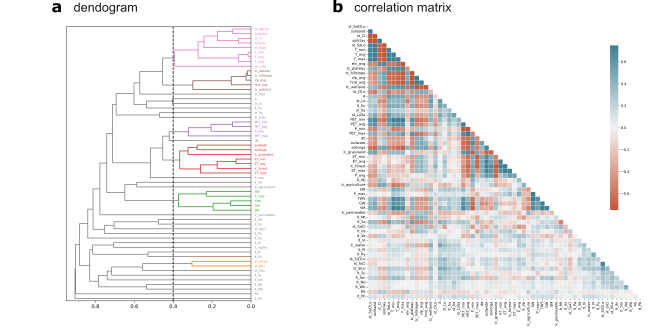
\includegraphics[width=0.98\linewidth]{figs/03_cluster.png}    
	\caption[Features correlation and clusters]
	{\textbf{---\;Feature analysis: correlation matrix and hierarchical clustering}.
	\textbf{a}\,--\,Correlation matrix, showing the absolute spearman correlation value, of the environmental predictors and target variables. 
        \textbf{b}\,--\,Dendogram representing the hierarchical relationship between the environmental predictors.
	}
    \label{fig:corrmatrix}            
\end{figure}

% ML models
\subsubsection{Machine Learning models} \label{sec:datagen:proceval:ml}

\par As outlined in Table \ref{tab:algorithms}, six machine learning (\texttt{ML}) models for regression were tested in this study. They are presented in this section aggregated in ascending order of complexity and computational demand, with the simpler models (first two) used as benchmarks for the more complex ones. Multiple Linear Regression (\texttt{MLR}) and Decision Trees (\texttt{DT}) were the first two models tested, followed by K-Nearest Neighbors (\texttt{KNN}), Support Vector Machines (\texttt{SVM}), Gradient Boosting Machine (\texttt{GBM}), and Random Forest (\texttt{RF}). For a comprehensive understanding of the models, including their mathematical foundations, see \cite{kuhn2013} and \cite{shalev2014}. 

% Insert Table
\FloatBarrier
\begin{table}[h]
    \centering
    \tiny
    \rowcolors{2}{white}{rowgray}
\begin{tabular}{p{4cm}p{1.5cm}p{1.5cm}p{2cm}p{1cm}p{1cm}}
\toprule
\textbf{Model}& \textbf{Complexity} & \textbf{Linear} & \textbf{Parametric} & \textbf{Missing Data} & \textbf{Intensive} \\
\midrule
Multiple Linear Regression (\texttt{MLR}) & Low & Linear & Parametric & \texttimes & \texttimes \\
Decision Trees (\texttt{DT}) & Low& Non-linear & Non-parametric & $\checkmark$ & \texttimes \\
K-Nearest Neighbours (\texttt{KNN}) & Medium & Non-linear & Non-parametric & \texttimes & $\checkmark$ \\
Support Vector Machines (\texttt{SVM}) & Medium& Non-linear & Parametric & \texttimes & $\checkmark$ \\
Gradient Boosting Machine (\texttt{GBM}) & High & Non-linear & Parametric & \texttimes & $\checkmark$ \\
Random Forest (\texttt{RF}) & High & Non-linear & Non-parametric & $\checkmark$ & $\checkmark$ \\
\bottomrule
\end{tabular}
\caption{Summary of Machine Learning models applied in the study.}
\label{tab:algorithms}
\end{table}

\par As mentioned above, we used Multiple Linear Regression (MLR) and Decision Trees (DT) as benchmark models. MLR is a straightforward machine learning model that presumes a proportional relationship between a dependent variable and all independent variables. Its objective is to identify a best-fit line for accurate prediction of the dependent variable, utilizing the Ordinary Least Squares method to minimize prediction errors. On the other hand, DT is a non-parametric model predicting the target variable's value through a tree-like structure. It segments data based on feature values until a specific criterion is reached, with predictions derived from the data characteristics of the leaf nodes. While DTs are interpretable and adept at handling complex feature interactions and missing data, they are susceptible to overfitting and can generate overly complex trees. In practice, this is often mitigated by using ensemble models like Random Forest and Gradient Boosting Machines.

\par In the intermediate complexity stage of our study, we employed K-Nearest Neighbours (\texttt{KNN}) and Support Vector Machines (\texttt{SVM}). \texttt{KNN} is a non-parametric model that bases its predictions on the $K$ nearest data points in the training set, without making assumptions about data distribution. It's applicable for both regression and classification, with predictions relying on the majority class among the $K$ neighbors. While \texttt{KNN} is straightforward to implement and adept at capturing complex feature relationships, it is computationally intensive and sensitive to hyperparameters like the value of $K$ and the chosen distance metric. \texttt{SVM}, on the other hand, is a linear model designed to find the optimal hyperplane that distinctively classifies data into different groups. It focuses on maximizing the margin between this hyperplane and the nearest data points from each class. Capable of managing non-linear relationships through kernel functions, which project data into higher dimensions, \texttt{SVM} is much used in fields like image and text classification, and bioinformatics. Nonetheless, its effectiveness hinges on the correct choice of hyperparameters like the kernel function and regularization parameter, and it requires significant computational resources for large datasets.

\par Finally we utilized the more complex Gradient Boosting Machines (\texttt{GBM}) and Random Forest (\texttt{RF}). \texttt{GBM} is an ensemble approach that amalgamates several weak models to form a potent predictive model. It progressively refines weak models based on the residual errors from preceding iterations, culminating in a prediction that combines all these models' outputs. \texttt{GBM} efficiently manages intricate feature interactions and generally exhibits greater resistance to overfitting compared to other tree-based models. However, it requires careful hyperparameter tuning, particularly in learning rate and tree count, and can be computationally demanding for extensive datasets. \texttt{RF}, another ensemble model, integrates multiple decision trees to forge a precise and robust prediction tool. It selects random feature and data point subsets for each tree, enhancing feature interaction capture and reducing overfitting risks. Predictions result from an aggregate of all trees' outputs, enhancing both accuracy and generalizability. While \texttt{RF} adeptly handles missing values and outliers, making it a popular choice in various applications, it also demands significant computational resources and offers less interpretability than individual decision trees.

\subsubsection{Hyperparameter tuning} \label{sec:datagen:proceval:partun}

\par The process of hyperparameter tuning was performed using a randomized search grid cross validation approach (\cite{bergstra2012} ). The approach consists of randomly  sampling hyperparameters from the \texttt{ML} model using a specified distribution and evaluating the performance of the model for each set of hyperparameters using cross-validation. This cross-validation here refers to the inner 10 folds used on the training set for each outer iteration, as outlined in the modeling overview. The best set of hyperparameters is then selected according to the model's overall performance. The performance metric here was chosen to $R^2$ (explained in Section \ref{sec:datagen:proceval:perform}). The set of distributions for each hyperparameter of each \texttt{ML} model is presented in Table \ref{tab:parameters}. It is important to note that, in order to reduce complexity, only the most sensible hyperparameters of the \texttt{ML} models were tested, the others remaining in default mode from the scikit-learn Python library. After the hyperparameters of the model were defined, the selected optimal model was fitted to the training data, and used to predict the results on the test data.

% Insert Table
\FloatBarrier
\begin{table}[h]
\centering
\tiny
\rowcolors{2}{white}{rowgray}
\begin{tabular}{p{3cm}p{3cm}p{3cm}}
\toprule
\textbf{Model} & \textbf{Parameter} & \textbf{Range$^*$}\\
\midrule
\texttt{MLR} & -- & --\\
\texttt{DT} & \texttt{max depth} & int(2, 20)\\
\texttt{DT} & \texttt{min samples leaf} & int(5, 100) \\
\texttt{KNN} & \texttt{leaf size} & int(1, 50) \\
\texttt{KNN} & \texttt{n neighbors} & int(1, 30) \\
\texttt{KNN} & \texttt{p} & int(1,5) \\
\texttt{SVM} & \texttt{gamma} & dbl(0.0001, 1)\\
\texttt{SVM} & \texttt{C} & dbl(1, 100)\\
\texttt{GBM} & \texttt{n estimators} & int(1, 500)\\
\texttt{GBM} & \texttt{max leaf nodes} & int(2, 100)\\
\texttt{GBM} & \texttt{learning rate} & dbl(0.01, 1)\\
\texttt{RF} & \texttt{n estimators} & int(1, 500)\\
\texttt{RF} & \texttt{max leaf nodes} & int(2, 100)\\
\bottomrule
\end{tabular}
\smallskip
    \parbox[t]{10cm}{\footnotesize
      \textit{$^*$ Legend: \\
      int: integer precision. \\ 
      dbl: double precision.}
    }
\caption{Ranges of hyperparameter values for tuning each \texttt{ML} model.}
\label{tab:parameters}
\end{table}

\subsubsection{Running times} \label{sec:datagen:proceval:runtim}

\par Model complexity certainly plays a role in the time taken to run the algorithm. In Table \ref{tab:runtime}, the time to run all the setup presented in the model pipeline section for each model is presented. The machine used to run the models was a i7-8700K CPU with 3.70GHz, 6 cores and 64GB RAM. Overall, comparing running times can give us a sense of the relative complexity of each model, but it's worth noting that the specific running time will depend on the size of the dataset, the complexity of the model, and the specific hyperparameters being used. \texttt{MLR} is the simplest model in the list and has the shortest running time by far, especially because this model doesn’t have hyperparameters to calibrate, which makes it even faster in the comparison. Other relatively time efficient model is \texttt{DT}, but still considerably more complex than linear regression. \texttt{KNN} and \texttt{SVM} come next in degree of complexity, taking between 2-4 minutes to run. Finally, \texttt{GBM} and \texttt{RF} are the most complex models in the list, which makes them considerably more computationally expensive than the other models, taking around 32 and 56 minutes, respectively.

% Insert Table
\FloatBarrier
\begin{table}[h]
\centering
\tiny
\rowcolors{2}{white}{rowgray}
\begin{tabular}{p{4cm}p{4cm}}
\toprule
\textbf{Model} & \textbf{Running time (mm:ss)}\\
\midrule
\texttt{MLR} & 00:02 \\
\texttt{DT}  & 00:14 \\
\texttt{KNN} & 02:28 \\
\texttt{SVM} & 04:01 \\
\texttt{GBM} & 31:57 \\
\texttt{RF}  & 55:53 \\
\bottomrule
\end{tabular}
\caption{Running times of each \texttt{ML} model.}
\label{tab:runtime}
\end{table}

\subsubsection{Performance of the individual models} \label{sec:datagen:proceval:perform}

\par After the processes covered in the previous section were performed in each one of the 10-fold combinations, the outcomes (resulting predictions and prediction intervals) could be evaluated. First, to assess the performance of the models, the following statistical metrics were used:
the percent bias (BIAS), in \%,
\begin{linenomath*}
\begin{equation}
\label{eq:bias}
\text{BIAS} = \frac{\sum (Q_{\text{pred}} - Q_{\text{obs}})}{\sum Q_{\text{obs}}} \times 100
\end{equation}
\end{linenomath*}
the Root Mean Squared Error (RMSE), in $\text{l}\cdot \text{s}^{-1}\cdot \text{km}^{-2}$ ,
\begin{linenomath*}
\begin{equation}
\label{eq:rmse}
\text{RMSE} = \sqrt{ \frac{\sum (Q_{\text{pred}} - Q_{\text{obs}})^2}{n}}
\end{equation}
\end{linenomath*}
and the coefficient of determination ($R^2$), dimensionless,
\begin{linenomath*}
\begin{equation}
\label{eq:r2}
R^2 = 1 - \frac{\sum (Q_{\text{pred}} - Q_{\text{obs}})^2}{\sum (Q_{\text{pred}} - \overline{Q}_{\text{obs}})^2}
\end{equation}
\end{linenomath*}
where $Q_{\text{obs}}$ is the observed unit discharge signature ($q_{m}$ or $q_{95}$), and $Q_{\text{pred}}$ is the predicted one.

\par The performance results of each \texttt{ML} model for $q_{m}$ and $q_{95}$ are presented in Figure \ref{fig:perf}. \texttt{MLR} and \texttt{DT} had good overall performance in predicting $q_{m}$, with statistical metrics equivalent of those from the other models. These two models had similar bias and RMSE, with \texttt{MLR} having better performance in $R^2$ for $q_{m}$ (0.81 against 0.77), and \texttt{DT} for $q_{95}$ (0.55 against 0.48). However, despite having a reasonable performance for $q_{95}$, they were considerably worse in comparison with the other models, especially looking at $R^2$. Regarding the remaining models (\texttt{KNN}, \texttt{SVM}, \texttt{GBM} and \texttt{RF}), \texttt{KNN} presented the worse results overall for both variables, whereas \texttt{SVM}, \texttt{GBM} and \texttt{RF} presented similar results for both variables, with \texttt{SVM} having a more pronounced bias towards underestimation.

\FloatBarrier
\begin{figure}[htb] % place figure in the page
	\centering                                       
	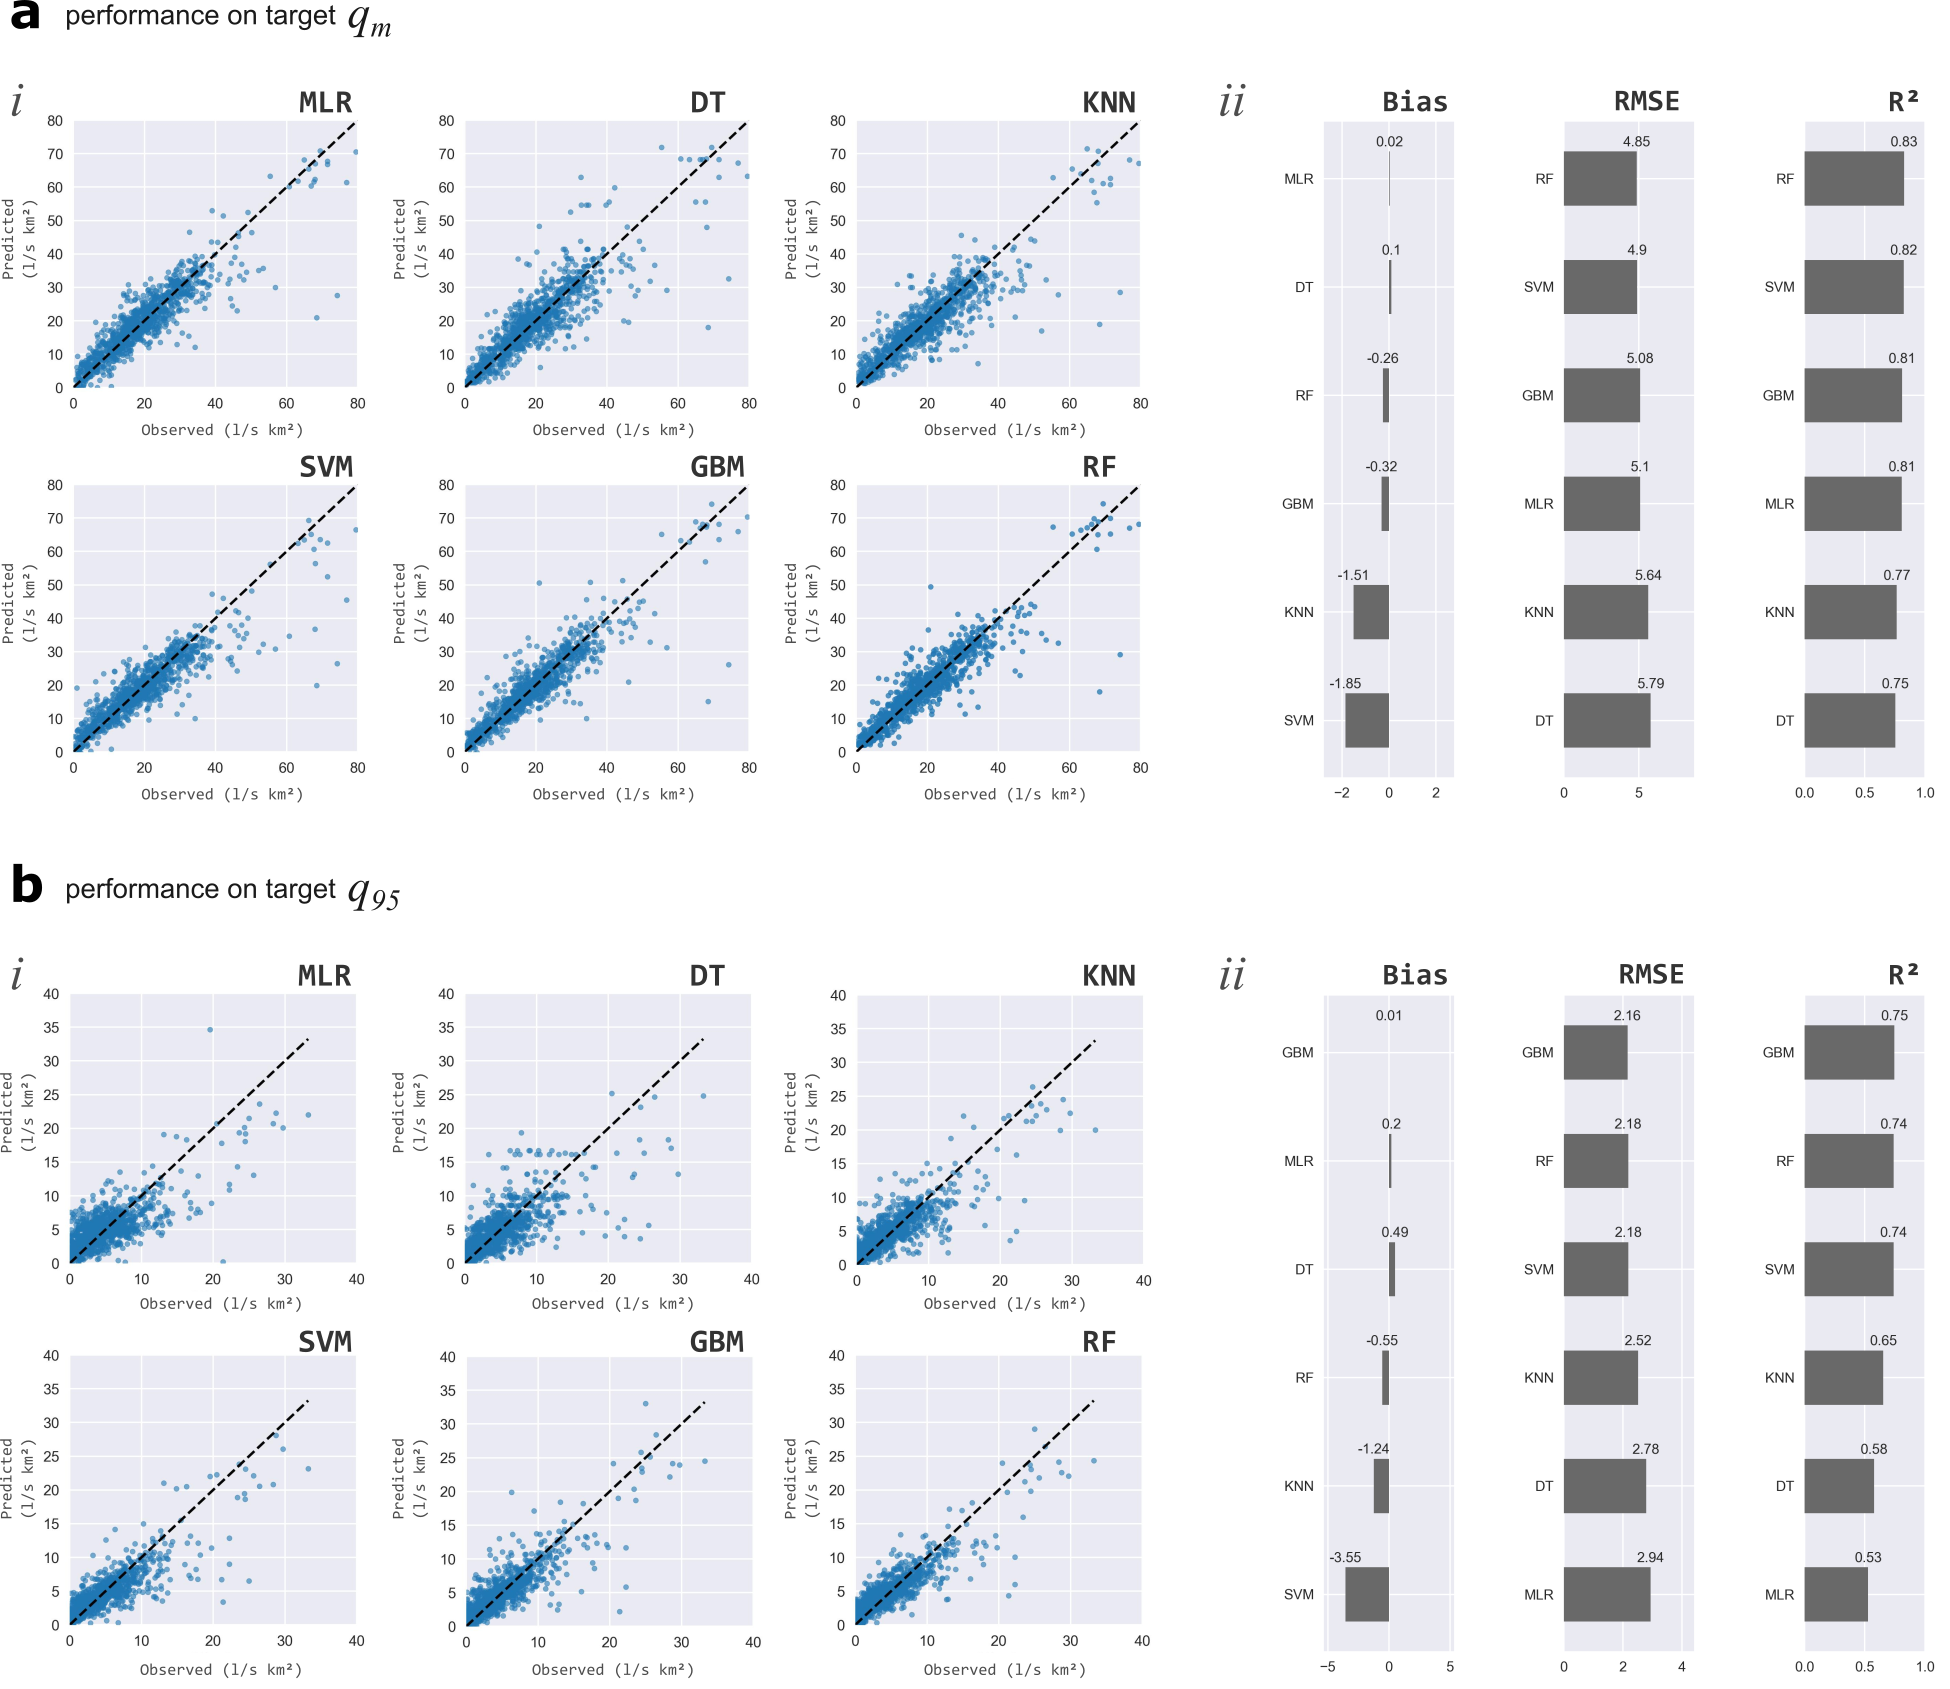
\includegraphics[width=0.98\linewidth]{figs/04_performance.png}    
	\caption[Performace of model evaluation]
	{ \textbf{---\;>>todo:legend Performace of \texttt{ML} model evaluation}.
		\textbf{a}\,--\,Tincidunt dui ut ornare lectus sit. Donec adipiscing tristique risus nec feugiat in fermentum posuere urna (detail \textrm{\textit{i}}).
		\textbf{b}\,--\,Tincidunt dui ut ornare lectus sit. Donec adipiscing tristique risus nec feugiat in fermentum posuere urna (detail \textrm{\textit{i}}).		
	}
	\label{fig:perf}  % use qualitative label                      
\end{figure}

\par In summary, all models evaluated here presented reasonable performances for both variables. For $q_{95}$, the simpler benchmark models (\texttt{MLR} and \texttt{DT}) performed considerably worse, and \texttt{RF} had a slightly better performance than \texttt{GBM} and \texttt{SVM} overall. In $q_{m}$, the added complexity didn’t seem to improve much the performance, and even a simple model such as \texttt{MLR} had a performance equivalent to much more robust models, such as \texttt{GBM} and \texttt{RF}, for this variable.

\subsubsection{Selection of the best model ensemble} \label{sec:datagen:proceval:best}

\par [Generic paragraph about ensemble theory and why it could be best than using a single model result]

\par In order to verify whether using ensemble predictions would enhance the results, different combinations of the models given in the previous section were tested for each target variable. The performance of difference combinations is given in **Table XX**. 

\par From the individual performances, we can see that SVM generally does not penalize the BIAS of the estimation. This, however, doesn't reflect in the other metrics, RMSE and R2, which indicates that it is more consistent in underestimating the results. 

\subsubsection{Feature importances} \label{sec:datagen:proceval:importance}

\par The importance of each predictor in the (\texttt{ML}) models was evaluated using permutation feature importance, a method outlined by \cite{altmann2010}. This approach involves assessing the model's performance when a single feature is randomly shuffled, with the importance measured by the loss in a performance metric. By shuffling a variable to random values, the resultant decrease in performance metric value indicates the importance of that variable. Permutation feature importance is particularly useful in analyzing black-box models, where it's challenging to discern how specific variables impact results. It offers a consistent standard for evaluating different models and accounts for all interactions between features, though it doesn't elucidate the nature of the relationship with the target variable. It's only useful in cases where correlated features are not present, because one correlated feature can mask the performance of another, underscoring the need to address multicollinearity before the processing phase.

\par The process starts by selecting a performance metric for the model, in our case \( R^2 \). The model's performance is then assessed on the test set to establish a baseline. Following this, the values of a single feature are permuted, and the model is re-trained and its performance is re-evaluated. The importance of a feature is determined by the difference in model performance with original and permuted feature values. This procedure is done for each features in the dataset, multiple times for each feature  to ensure that the model's performance isn't influenced by random data (the number of times used here was 10). The feature's importance score is then derived from the average performance decrease across these iterations.

\par Re-training the model on shuffled features is not mandatory and can significantly increase computation time. However, despite the lack of official recommendations in the literature, we argue that this step is essential for accurate analysis. Without allowing the model to re-train on shuffled features, performance metrics are overestimated. This overestimation occurs because the model is not given the opportunity to utilize other features to compensate for the information loss caused by shuffling. Re-training ensures that the model adapts to the altered feature set, providing a more realistic measure of each feature's importance. By doing so, we obtain a clearer understanding of how the model performs when certain features are disrupted, leading to more robust and reliable interpretations. Ultimately, this step enhances the overall validity and trustworthiness of the real importance of each feature in the model's performance.

\par In Figure \ref{fig:importance} are presented the importances of the 15 most important features for $q_{m}$ and $q_{95}$, respectively. The values reflect the decrease in $R^2$ value after randomly shuffling the selected variable. Overall, the average climatological precipitation ($p_{\text{avg}}$) was the most important predictor for both target streamflow signatures. Its importance is pronounced, where other variable importances seem to be more evenly distributed for both target variables. A slightly greater contribution than other remaining variables is also seen in organic content in soils ($SC_{org}$), and, for $q_{95}$ exclusively, drainage density ($DEM_{dd}$) also had a fair contribution in the performance.

\FloatBarrier
\begin{figure}[htb] % place figure in the page
	\centering                                       
	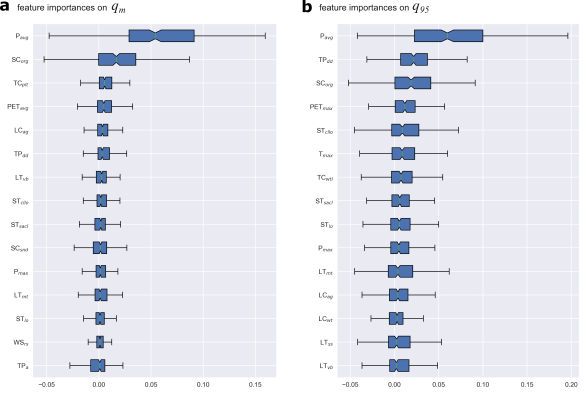
\includegraphics[width=0.98\linewidth]{figs/05_importance.png}    
	\caption[Importance of features]
	{ \textbf{---\;>>todo:legend}.
		\textbf{a}\,--\,Tincidunt dui ut ornare lectus sit. Donec adipiscing tristique risus nec feugiat in fermentum posuere urna (detail \textrm{\textit{i}}).
		\textbf{b}\,--\,Tincidunt dui ut ornare lectus sit. Donec adipiscing tristique risus nec feugiat in fermentum posuere urna (detail \textrm{\textit{i}}).		
	}
	\label{fig:importance}  % use qualitative label                      
\end{figure}

\subsubsection{Uncertainty estimation} \label{sec:datagen:proceval:uncert}

\par \textcolor{red}{TODO}:
\begin{itemize}
  \item Figure of insights on predicted rather than observed
  \item Only for ENSEMBLE
  \item Figures on the estimation/extrapolation method
\end{itemize}

\par The assessment of uncertainty provided various insights into the distribution and structure of errors. The panels in Figure \ref{fig:uncert}a and Figure \ref{fig:uncert}b display the visualizations used for the best ensemble \texttt{ML} model adjusted for target variables $q_{m}$ and $q_{95}$, respectively. The first three charts visually present the structure of the residuals: the first chart shows the residuals as a function of the magnitude of the predicted variable, the second is a histogram of the residuals, and the third is the Quantile-Quantile plot, which relates the empirical quantiles obtained with the expected quantiles for a normal distribution. The fourth chart, vertically aligned with the residual chart, depicts the accumulated variance $\sigma^2$ as a function of the magnitude of observed values. This visualization is particularly informative, as if the residuals emerge from a random process (i.e., with independence), the variance should quickly stabilize around a constant value as the number of samples increases.

\par The residual structure charts reveal that the residuals are relatively well-centered around zero, with very low means. However, this symmetry in the mean does not imply structural symmetry, as positive residuals tend to be larger for higher predicted values, indicating that the \texttt{ML} models generally underestimate higher reference flows. The Quantile-Quantile charts reinforce this observation, as the upper tail mostly presents a more pronounced curve, reaching higher values (around 50 l/s km$^2$) on the positive side.

\par Based on the analysis presented in the charts from Figure \ref{fig:uncert}, it was hypothesized that the error is linearly proportional to the magnitude of the predicted value. To test this assumption, two steps were performed:

\subparagraph a the data were divided into deciles based on the predicted values, resulting in approximately 110 samples per 10\% quantile interval. For each interval, the error ranges that encompass 90\% (between the 0.05 and 0.95 quantiles) and 75\% (between the 0.125 and 0.875 quantiles) of the errors were computed.

\subparagraph b Quantile Regression (\texttt{QR}) models were employed on the same quantiles, with the predicted discharges being used as independent variables, and the error associated as the dependent ones.

\par A \texttt{QR} model works in a similar manner than linear regression, with the main difference being it uses a specified quantile instead of the mean of the dependent variable as a focus, e.g. by using a quantile of 0.95, the model returns a line of which 95\% of values would be below. Therefore, if our assumption is correct, the lines generated by QR models would cross the decile points in about the same value.

\par Figures XXXXX show the distribution of errors in relation to the predicted values, with the empiric quantiles at every decile break point, and the \texttt{QR} fitted models. [general description of the behaviour of the plots]

\par This approach, despite being rather simplistic - by considering the error only as a function of the predicted values - possesses a hidden robustness: as the predicted value is a function of all environmental variables.

\par [continue text here with rationality and presentation of the final estimation]

\FloatBarrier
\begin{figure}[t] % place figure in the page
	\centering                                       
	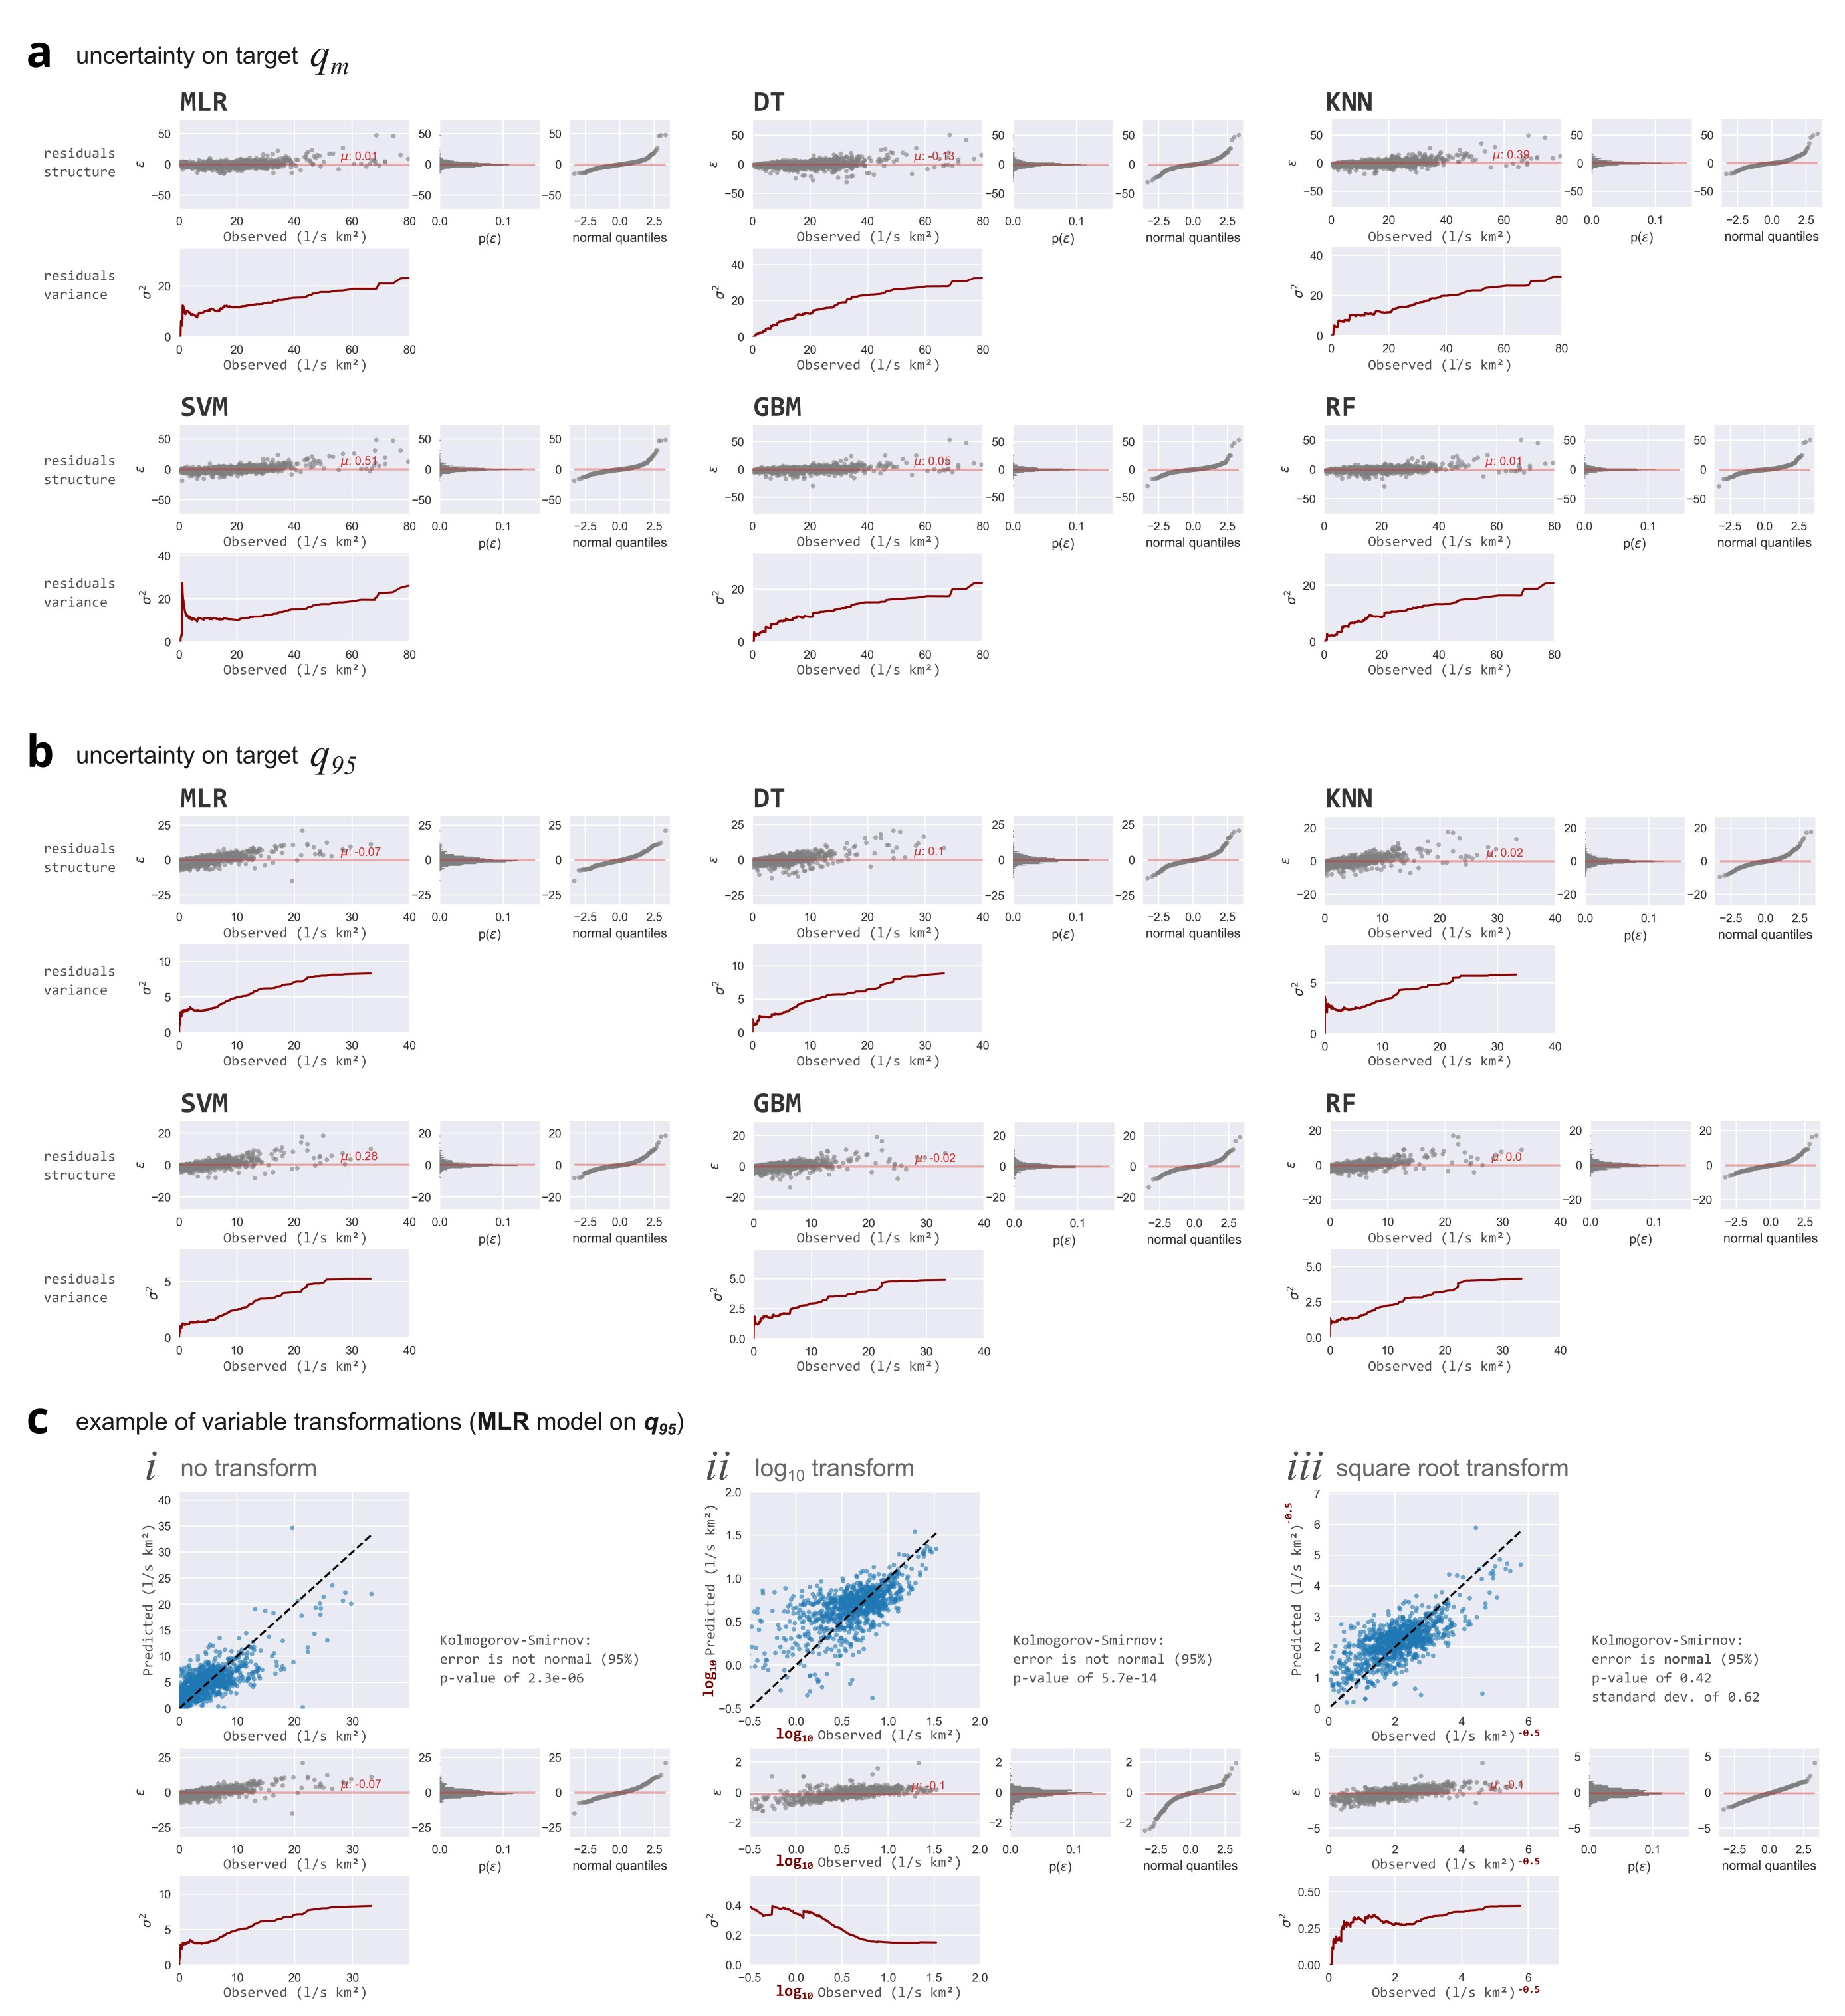
\includegraphics[width=0.98\linewidth]{figs/uncertainty.jpg}    
	\caption[Insights into Uncertainty]
	{\textbf{---\;Insights into Uncertainty from Residuals Analysis}.
        \textbf{a}\,--\,Analysis of uncertainty for the target variable $q_m$, revealing the structure of residuals $\epsilon$ (including distribution, histogram, and Quantile-Quantile plot) and examining the stability of accumulated variance $\sigma^2$ for each Machine Learning model.
        \textbf{b}\,--\,Analysis of uncertainty for the target variable $q_{95}$, revealing the structure of residuals $\epsilon$ (including distribution, histogram, and Quantile-Quantile plot) and examining the stability of accumulated variance $\sigma^2$ for each Machine Learning model.
        \textbf{c}\,--\,Variable transformations applied in the \texttt{MLR} model for the target variable $q_{95}$ included: no transformation (detail \textrm{\textit{i}}); logarithmic transformation (detail \textrm{\textit{ii}}); and square root transformation (detail \textrm{\textit{iii}}). The square root transformation was the only method that passed the Kolmogorov-Smirnov test.
        }
	\label{fig:uncert}  % use qualitative label                      
\end{figure}

% Dataset covering all Brazilian unit catchments
\subsection{Output dataset} \label{sec:datagen:dataset}

\par With all the insights taken from ML modeling process and evaluation described in the previous section, a final dataset, and the main goal of this study, was produced. The dataset consists of qm and q95 values for all the river segments in the domain together with uncertainty estimations. The segments were selected from a subset of the BHO 5k dataset, which includes rivers that are in or drain to Brazil, and excludes island rivers. In other words, the dataset domain covers the Brazilian continent and the Amazon River basin.

\par The processing of this dataset consisted of the following steps:

\begin{enumerate}

\item Each selected \texttt{ML} model from the ensemble evaluation (section \ref{sec:datagen:proceval:best}) was trained using all environmental descriptors in a 10-fold CV approach to calibrate the hyperparameters on all gauged data.

\item For each one of the models, results were computed for all stream segments in the domain, which included gauged and ungauged data, and the predictions were then averaged to produce one final value for each target variable.

\item The 90\% and 75\% confidence intervals, i.e. the uncertainty measures, was computed using the \texttt{QR} functions computed in section \ref{sec:datagen:proceval:uncert}.

\end{enumerate}

\par Different from the evaluation process, all features available were used. As the process of feature selection was mainly used to assess the influence of the features in the models - i.e. reducing multicollinearity between features for evaluating their influence in the predictions, not to make the predictions better - for producing the final dataset, it was considered best to use all features available, as there could have been minimal improvements in adding features that were not captured in the evaluation process. These differences, however, should be minimal according to evaluation presented herein (section \ref{sec:datagen:proceval}. As it is unlikely that using more features can worsen the performance of a model, because \texttt{ML} models can automatically capture which variables have more influence in the target variable and then apply low weights to them, the only reason for using less variables would be for reducing computation times, which would only be significant if the application had thousands of features.

\par Another main difference for the production phase in contrast with the evaluation phase was that the training-predict pipeline was used only once for each model-target pair. In the evaluation, we used a nested k-fold framework for all gauged points to be applied as training and test data instead of just one train-test split, where the inner folds were used to calibrate the hyper-parameters on each training set, and the outer folds just to evaluate the models on an  unseen test set. This framework in the evaluation process gave more robustness in the results evaluated, as each model was trained and validated 100 times, and tested 10 times. For ungauged data, however, as there is no test to be performed, the most robust pipeline consists of using all data available for training and calibrate the models, i.e. the inner folds, and then applying the models at the ungauged sites, i.e. the outer fold.


\section{Data availability}\label{dataav}

\par Data is available at [...]. >>todo: links and more options.

\par For data processing and modeling, we utilized the scikit-learn library in Python.

% Discussion and conclusions
\section{Discussion and conclusions} \label{discussion}

% Implications
\subsection{Summary of achievements and limitations of this research} \label{discussion:dataset}

\par This study aimed to produce a dataset with information of signature average ($q_{m}$) and low ($q_{95}$) flows for all river stretches in the Brazilian territory, and some of the main South American rivers, using state-of-the-art machine learning (\texttt{ML}) algorithms to achieve this goal. It was built on top of a vector river network, where corresponding catchments of each river stretch were used to collect environmental data and compute the target signature flows. The final dataset was produced after careful evaluation of the \texttt{ML} models at selected gauging stations, and the best models were selected to produce the final values in the whole domain.

\par The final dataset produced by this unprecedented application has the potential of a myriad of uses. It can be used as support information in policy making, environmental conservation, agriculture, and infrastructure development. Additionally, it offers valuable insights for hydrological studies, climate change impact assessments, and water resource management strategies across Brazil.

\par Moreover, this research provided a fair comparison of some of the most used machine learning models in the literature, and proposed crucial steps in the modeling pipeline that have been overlooked in other similar hydrological applications of similar nature. These include model-agnostic feature clustering for importance computation that accounts for removing multicolinearity between features, and confidence interval computation based on uncertainty models. These methodological approaches ensure that the dataset is robust and the findings are reliable, offering a more nuanced understanding of river flow dynamics. It is expected that these innovations will be considered in future studies.

\par For this study, we used the best possible environmental data available that would be consistent for whole Brazilian region. These data, despite having its associated uncertainties, generally reflects the behaviour of the catchments analyzed. Still, it is important to address that this dataset posses its limitations, which will be covered over the next paragraphs.

\par First, the spatial distribution of the gauged data used for training and testing was not even. In southeast and south regions of the country, much more gauging data were available, with very few stations in northeast and in Amazon regions. This uneven distribution may lead to biases in the model, as regions with sparse data are less represented in the training process, potentially affecting the accuracy of flow estimates in those areas.

\par Additionally, some environmental descriptors were only accounted in terms of averages for the whole catchment areas. This was the case for elevation, slope, and height above nearest drainage. The inclusion of the variance of these data within a catchment is not straightforward. This simplification might overlook important sub-catchment variations that could influence flow characteristics.

\par Finally, some environmental information was not included in the modeling process, mainly due to difficulties in obtaining those at such scale. This is the case for drainage geomorphological information, such as river width, depth, and slope. The exclusion of those could have affected the accuracy of flow estimations.

\subsection{Interpretation of findings} \label{discussion:findings}

\par Based on the interpretation of the model evaluation process, we can highlight that (1) For estimating average streamflow in ungauged locations, the complexity of the model used didn’t yield a significant improvement in the results, and average precipitation alone could give reasonable estimates. (2) For low flows, besides average precipitation, other data become more important, such as soil organic content, minimum precipitation and elevation; and more robust non-linear models have a better performance. And (3) the quality of environmental data is the most valuable asset for such applications, regardless of the model. As these applications were made very easy by recent developments, studies should focus more on targeting the preparation and investigation of the data. Processes such as multi-collinearity analysis and feature selection should receive more attention, which is not the case in most studies to date. By improving the quality and granularity of input data, the robustness and reliability of flow predictions can be significantly enhanced.

\par The results suggest that machine learning models can be effective in predicting streamflow for both $q_{m}$ and $q_{95}$, and also highlight the importance of carefully selecting and tuning the models to achieve optimal performance, as well as the need for high-quality data to feed them. The performance of the models can vary depending on the specific model used. More robust models, such as \texttt{GBM} and \texttt{RF}, had similar results than simpler models such as \texttt{MLR} or \texttt{DT} for $q_{m}$, and only slightly better results for $q_{95}$ when comparing with a much less complex \texttt{SVM}. For $q_{95}$, in particular, the simplicity of \texttt{MLR}, \texttt{DT} and \texttt{KNN} yield reasonable results, with $R^2$ between 0.48 to 0.66, although a quite significant improvement was achieved with \texttt{SVM} (with $R^2$ of 0.74), and an improvement in bias by the incremented complexity of \texttt{GBM} and \texttt{RF}.

\par Regarding the importance of the features, it’s not much surprising that average precipitation is the most important predictor overall for both target variables. Still, for the case of predicting low flows ($q_{95}$), drainage density ($Dd$) and organic content in soils ($SC_org$) gained more meaningful contributions in the models' predictions. Drainage density, more impressively, had a correlation coefficient with $q_95$ of only -0.06, which highlights the non linearity of this influence and the complex interactions of the system.

\par The reasons behind these variables' influences in controlling low flows is beyond the scope of this study. This is likely due to the complex interactions over time and the coevolution of the landscape, where soil and drainage channeling properties affect and are affected by the magnitude of flows in drier periods, making them a good proxy for predicting those. These relationships could be further investigated in future research. Moreover, improving the accuracy of these data by targeting more resources in the acquisition of these data at larger scales should help to improve low-flow estimations even further.

\par It's also worth mentioning that $SC_org$ was the representative variable of a cluster of variables that included soil water content ($SC_wat$), grassland and forest occupation rates ($LC_forest$ and $LC_grassland$), and all related to evapotranspiration ($ET_avg$, $ET_min$, and $ET_max$). The fact that these variables were grouped this way is not always obvious. The main assumption with the process of hierarchical clustering is that one variable of the cluster can be used to predict the other(s), and that the selection of any of the variables from the cluster would not yield significantly different results, because all variables within a cluster are highly correlated. Of course, the distance criterion for cluster separation is subject to analysis, and our criterion here was that no selected variable would have pair-wise spearman correlation above 0.7. Still, it was not tested whether (1) using different thresholds would result in different model performances, nor (2) using a different variable from each cluster would impact the results.

\par Regarding the uncertainty of the results, it is important to note the substantial challenge in knowing exactly how wrong is an estimation. Several sources contribute to the overall inaccuracy and imprecision, from the collection of the target data itself, including measuring and deriving rating curves, to all random, epistemic, and systematic errors associated with environmental descriptors. In this study, we focused on looking for patterns in the error associated with the data. Although the exact nature of these errors remains uncertain, we proposed an "error model" and successfully fitted the observed errors to this model. This model involved simple regressions on the quantiles of the predicted values relative to the associated errors, under the assumption that errors are proportional to the magnitude of the values.

\par The degree of uncertainty in estimations can vary significantly depending on environmental conditions. For instance, in regions experiencing heavy rainfall, the error in predicting flow rates tends to be smaller because rainfall alone predominantly dictates the magnitude of flow. This direct relationship simplifies the estimation process, leading to more precise predictions. Conversely, in drier regions, other environmental factors have larger influence on flows, making it more challenging to determine the exact cause of fluctuations in flow rates. As a result, the relative uncertainty is likely higher due to the complex interplay of variables, making accurate predictions more difficult. That was observed here, as relative errors were smaller at higher flow rates.

% Comparison with previous studies
\subsection{Comparison with similar studies} \label{discussion:similar}

\par The potential of \texttt{ML} models in hydrological research is recognized as being vast. Still, its use is quite recent, and not many application have been found in the literature so far. Of the studies analyzed in this research, three had a similar approach than this one, i.e. attempted to use \texttt{ML} models to predict streamflow signatures: one for peak event flows over the United States (\cite{potdar2021}), one for low flows comprising around 200 basins in the southern USA (\cite{worland2018}), and one for average and low flows in the Doce River basin in Brazil (\cite{ferreira2021}). There are a few points that are worth discussing about these studies in relation to the one presented herein, regarding mostly the model inter-comparisons and the process of feature selection and importance computation.

\par In the two studies that compared the performances of linear models, such as \texttt{MLR}, with more robust state-of-the-art \texttt{ML} models (\cite{ferreira2021, worland2018}), both found the predictions of linear models being much worse than more complex models, which is contrasting with the results found here, where a linear structure was similar to a more complex structures for mean flows, and only worse for low flows albeit having reasonable estimates. Both studies used similar environmental predictors, as well as of cross-validation and hyperparameter tuning, with small differences in comparison with this study. The main difference relies on the process of filtering the data that is being used by the models. Still, the process of feature selection shouldn’t be the reason for considerable decrease in performance, as this process is performed with the main goals of reducing running times and removing multi-collinearity for later assessing variable importances.

\par Regarding the importances of the predictors, in all three studies mentioned in this discussion this process is performed without the adequate feature selection to reduce multi-collinearity. Reducing multi-collinearity is essential for feature importance computation, because if there are two correlated variables, one will compensate for the absence of the other, and so both of them will have their importances drastically underestimated. Despite that, in \cite{worland2018} and \cite{potdar2021}, no process of feature selection is performed. In \cite{ferreira2021}, the authors removed variables with pair-wise pearson correlation below 0.95, which is a very high threshold (recommended values in the literature vary from 0.6 to 0.8), and later performed recursive feature elimination (RFE), which is a process that requires importance computation to remove non-important features, and should only be performed in non-collinear data. Because of those methodological flaws, all analyses regarding variable importances in those studies won’t be considered for comparison with this study.


\section*{CRediT authorship contribution statement}

\textbf{Rafael Barbedo}: Conceptualization, Methodology, Writing - original draft. \textbf{Iporã Possantti}: Investigation, Visualization, Formal analysis, Writing - review and editing. \textbf{Mino Sorribas}: Methodology, Investigation, Formal analysis, Writing - review. \textbf{Rodrigo Paiva}: Project administration, Funding acquisition Writing - review. \textbf{Walter Collischonn}: Conceptualization, Methodology, Supervision, Writing - review.

\section*{Acknowledgements}

\noindent \par The authors would like to acknowledge the financial support provided by the Brazilian National Water and Sanitation Agency (ANA) in the context of the project \say{Technological Cooperation for Hydrological Assessments in Brazil - Streamflow regionalisation} (grant number: TED-05/2019-ANA), the Google LLC for making available the Google Earth Engine (GEE) platform, and all data providers for the global products used in this study.

\section*{Declaration on competing interest}

\noindent The authors declare that they have no known competing financial interests or personal relationships that could have appeared to influence the work reported in this paper.

\section*{Declaration of generative AI and AI-assisted technologies}

\noindent During the preparation of this work the authors used \texttt{CHAT-GPT 4.0} in order to improve language and readability. After using this tool, the authors reviewed and edited the content as needed and take full responsibility for the content of the publication.

	
% ---------------- Appendix ----------------
\clearpage
\begin{appendices}
	
\section{The Appendix} \label{ap:first}

\par >>todo: appendix -- database figure(s) and description.

\par \textcolor{red}{Nam blandit dui quis nunc pretium, sed egestas felis mattis. Aenean tristique, massa non vestibulum pulvinar, justo ante efficitur turpis, vitae feugiat sem nisi ut arcu. Lorem ipsum dolor sit amet, consectetur adipiscing elit. Nunc rhoncus lacus nisi, id efficitur ligula placerat quis. Maecenas sit amet mi aliquam, congue metus a, accumsan leo. Vivamus id lobortis libero, ac fermentum ligula. In sollicitudin, enim varius rhoncus feugiat, odio lectus interdum enim, a posuere nunc magna eget nisi. Sed eget lacus et ante mollis sollicitudin quis varius velit. Aenean sit amet ipsum rhoncus eros iaculis ornare. Phasellus nec tortor ultrices orci sollicitudin fermentum. Mauris mattis nibh dui, a condimentum mi fermentum sed. Aliquam ac tempor mi. Fusce ac libero pharetra, sagittis metus id, dictum massa. Vestibulum ante ipsum primis in faucibus orci luctus et ultrices posuere cubilia curae; Sed a erat accumsan, interdum leo sed, porttitor risus.}

\begin{figure}[t!] % place figure in the page
	\centering                                       
	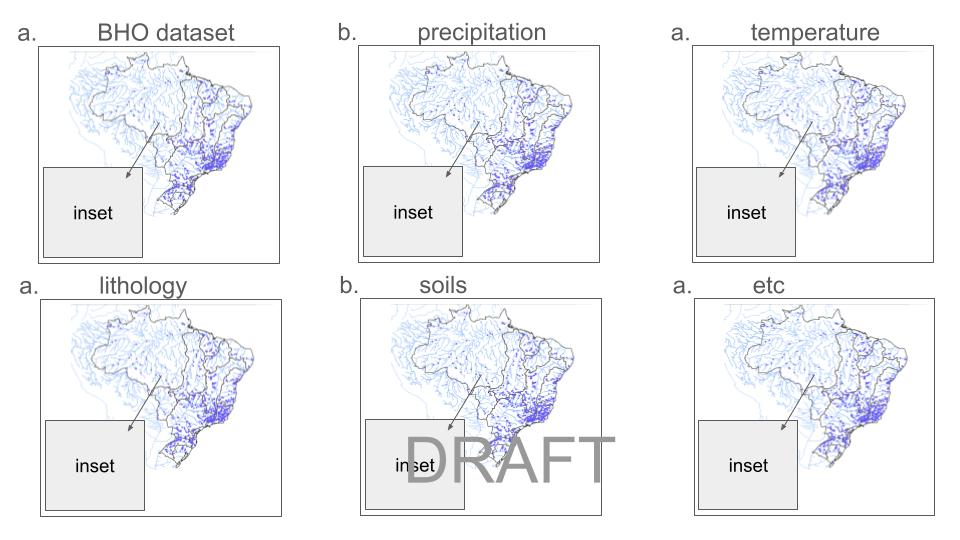
\includegraphics[width=0.98\linewidth]{figs/pre_descrip.jpg}    
	\caption[>>:todo:caption Short caption]
	{ \textbf{---\;>>todo:caption This is the long caption}.
		\textbf{a}\,--\,Tincidunt dui ut ornare lectus sit. Donec adipiscing tristique risus nec feugiat in fermentum posuere urna (detail \textrm{\textit{i}}).
		\textbf{b}\,--\,Tincidunt dui ut ornare lectus sit. Donec adipiscing tristique risus nec feugiat in fermentum posuere urna (detail \textrm{\textit{i}}).		
	}
	\label{fig:descript}  % use qualitative label                      
\end{figure}


\clearpage

\end{appendices}
% print references
\clearpage
\singlespacing
\printbibliography
\end{document}
	
